\documentclass[epsf,a4paper]{article}
\usepackage{html, graphics}
\newcommand{\oofem}{\htmladdnormallink{OOFEM}{http://www.oofem.org}\ }
\newcommand{\bp}{\htmladdnormallink{Bo\v{r}ek Patz\'{a}k}{http://mech.fsv.cvut.cz/~bp/bp.html}}
\newcommand{\mbf}[1]{\mbox{\boldmath$#1$}}
\newcommand{\descitem}[1]{{\noindent \bf #1}}
\newcommand{\elemkeyword}[1]{\descitem{Keyword}~{\em #1}}
\newcommand{\elemparam}[2]{{{#1\tiny (#2)}~\#}}
\newcommand{\optelemparam}[2]{[{~\elemparam{#1}{#2}}]}
\newcommand{\param}[1]{{\it #1}}
\newcommand{\optparam}[1]{[{\it #1}]}
\newcommand{\be}{\begin{equation}}
\newcommand{\ee}{\end{equation}}
\newcommand {\bea}{\begin{eqnarray}}     
\newcommand {\eea}{\end{eqnarray}}       
\newcommand {\bsig}{\mbf{\sigma}}
\newcommand {\alphaPsi}{\alpha_{\psi}}
\newcommand {\kappac}{\kappa_{\mathrm{c}}}
\newcommand {\tauY}{\tau_{\mathrm {Y}}}
\newcommand {\eps} {\mbf{\varepsilon}}
\newcommand {\epsp} {\eps_{\mathrm{p}}}
\newcommand {\epspd} {\dot{\eps}_{\mathrm{p}}}
\newcommand{\ignore}[1]{}
\newcommand{\del}[2]{\mbox{$\displaystyle\frac{#1}{#2}$}}
\newcommand{\ep}[0]{\mbf{\varepsilon}^p}
\newcommand{\epd}[0]{\dot{\mbf{\varepsilon}}^p}
\newcommand{\e}{\mbf{\varepsilon}}
\newcommand{\sig}{\mbf{\sigma}}
\newcommand{\kap}{\mbf{\kappa}}
\newcommand{\ve}{\mbf{e}}             % vector e
\newcommand{\vet}{\tilde{\ve}}
\newcommand{\veps}{\mbf{\varepsilon}}        % vector epsilon
\newcommand{\vsig}{\mbf{\sigma}}             % vector sigma
\newcommand{\vs}{\mbf{s}}             % vector s
\newcommand{\vepst}{\tilde{\veps}}
\newcommand{\vst}{\mbf{s}^T}          % vector s transposed 
\newcommand{\vsigt}{\tilde{\vsig}}
\newcommand{\dvepst}{\delta\tilde{\veps}}
\newcommand{\dvet}{\delta\vet}
\newcommand{\dvs}{\delta\vs}
\newcommand{\dvsig}{\delta\vsig}
\newcommand{\dO}{\,\mbox{d}\Omega}
\newcommand{\sym}{_{\mbox{\small sym}}}
\newcommand{\vxi}{\mbf{\xi}}             % vector xi
\newcommand{\quarter}{\mbox{$\frac{1}{4}$}}
\newcommand{\vx}{\mbf{x}}             % vector x


\begin{document}
%begin{latexonly}
\title{\oofem Material Model Library Manual}
\author{\bp \\ \\
Czech Technical University\\
Faculty of Civil Engineering\\
Department of Structural Mechanics\\
Th\'akurova 7, 166 29 Prague, Czech Republic
}
\maketitle
%end{latexonly}
\begin{htmlonly}
\begin{center}
{\Large \oofem Material Model Library Manual}\\ \\
{\bp \\ 
Czech Technical University\\
Faculty of Civil Engineering\\
Department of Structural Mechanics\\
Th\'akurova 7, 166 29 Prague, Czech Republic
}
\end{htmlonly}

\newpage
\tableofcontents
\listoftables
\section{Material Models for Structural Analysis}
\subsection{Linear Elastic Materials}
\subsubsection{Isotropic Linear Elastic Material}
\label{IsoLE}
Linear isotropic material model. The model parameters are summarized
in table~\ref{IsoLE_table}.

\begin{table}[h]                                                                
%\begin{center}                                                                  
\begin{tabular}{|l|p{9cm}|}                                                      
\hline                                                                          
Description & Linear isotropic elastic material\\
\hline                                                                          
Record Format & \descitem{IsoLE} \elemparam{num}{in}
\elemparam{d}{rn} \elemparam{E}{rn} \elemparam{n}{rn}
\elemparam{tAlpha}{rn}\\
Parameters &- \param{num} material model number\\
&- \param{d} material density\\
&- \param{E} Young modulus\\
&- \param{n} Poisson ratio\\
&- \param{tAlpha} thermal dilatation coefficient\\
Supported modes& 3dMat, PlaneStress, PlaneStrain, 1dMat,
2dPlateLayer, 2dBeamLayer, 3dShellLayer, 2dPlate, 2dBeam, 3dShell,
3dBeam, PlaneStressRot\\
Features & Adaptivity support\\
\hline
\end{tabular}                                                                   
\caption{Linear Isotropic Material - summary.}                
\label{IsoLE_table}                                                         
%\end{center}                                                                    
\end{table}                                                                     


\subsubsection{Orthotropic Linear Elastic Material}
\label{OrthoLE}
Linear orthotropic, linear elastic  material model. The model parameters are summarized
in table~\ref{OrthoLE_table}.
Local coordinate system, which determines axes of material orthotrophy
can by specified using \param{lcs} array. This array contains six numbers,
where first three numbers represent directional vector of local
x-axis, and next three numbers represent directional vector of local
y-axis. The local z-axis is determined using vector product. 
The right-hand coordinate system is assumed. Local coordinate system
can also be specified using \param{scs} parameter. Then local coordinate
system is specified in so called ``shell''
coordinate system, which is defined locally on each particular element
and its definition is as follows: principal z-axis is perpendicular to
shell mid-section, x-axis is perpendicular to z-axis and normal to
user specified vector (so x-axis is parallel to plane, with  being
normal to this plane) and y-axis is perpendicular both to x and z
axes. This definition of coordinate system can be used only with plates
and shells elements. 
When vector  is parallel to z-axis an error occurs. The \param{scs} array contain three numbers
defining direction vector . If no local coordinate system is
specified, by default a global coordinate system is used. 

For 3D case the material compliance matrix has the following form
\begin{equation}
  \mbf{C}=\left[\begin{array}{cccccc}
      1/E_X & -\nu_{xy}/E_x& -\nu_{xz}/E_x& 0& 0&0\\
      -\nu_{yx}/E_y & 1/E_y& -\nu_{yz}/E_y& 0& 0&0\\
      -\nu_{zx}/E_z & -\nu_{zy}/E_z& 1/E_z& 0& 0&0\\
      0 & 0 & 0 & 1/G_{yz} & 0 & 0\\
      0 & 0 & 0 & 0 & 1/G_{xz} & 0\\
      0 & 0 & 0 & 0 & 0 & 1/G_{xy}
    \end{array}\right]
\end{equation}
By inversion, the material stiffness matrix has the form
\begin{equation}
  \mbf{D}=\left[\begin{array}{cccccc}
      d_{xx} & d_{xy} & d_{xz} & 0 & 0 & 0\\
      & d_{yy} & d_{yz} & 0 & 0 & 0\\
      \rm {sym} & & d_{zz} & 0 & 0 & 0\\
      0 & 0 & 0 & G_{yz} & 0 & 0\\
      0 & 0 & 0 & 0 & G_{xz} & 0\\
      0 & 0 & 0 & 0 & 0 & G_{xy}
    \end{array}\right]
\end{equation}
where $\xi=1-(\nu_{xy}*\nu_{yx}+\nu_{yz}*\nu_{zy}+\nu_{zx}*\nu_{xz})-(\nu_{xy}*\nu_{yz}*\nu_{zx}+\nu_{yx}*\nu_{zy}*\nu_{xz})$ and
\begin{eqnarray}
  d_{xx}&=&E_X(1-\nu_{yz}*\nu_{zy})/\xi,\\
  d_{xy}&=&E_y*(\nu_{xy}+\nu_{xz}*\nu_{zy})/\xi,\\
  d_{xz}&=&E_z*(\nu_{xz}+\nu_{yz}*\nu_{xy})/\xi,\\
  d_{yy}&=&E_y*(1-\nu_{xz}*\nu_{zx})/\xi,\\
  d_{yz}&=&E_z*(\nu_{yz}+\nu_{yx}*\nu_{xz})/\xi,\\
  d_{zz}&=&E_z*(1-\nu_{yx}*\nu_{xy})/\xi.  
\end{eqnarray}


 $E_i$ is the Young's modulus in the $i$-th direction, $G_{ij}$ is the shear modulus in $ij$ plane, $\nu_{ij}$ major Poisson's ratio, and $\nu_{ji}$ minor Poisson's ratio. Assuming that $E_x>E_y>E_z$, $\nu_{xy} > \nu_{yx}$ etc., then the $\nu_{xy}$ is refered to as major Poisson's ratio, while $\nu_{yx}$ refered as minor Poisson's ratio.
Note, that there is only nine independent material parameters,
because of symmetry conditions. The symmetry condition yields
$$\nu_{xy}E_y=\nu_{yx}E_x,\ \ \nu_{yz}E_z=\nu_{zy}E_y,\ \ \nu_{zx}E_x=\nu_{xz}E_z$$
The model description and parameters are summarized
in table~\ref{OrthoLE_table}.

\begin{table}[h]                                                                
%\begin{center}                                                                  
\begin{tabular}{|l|p{9cm}|}                                                      
\hline                                                                          
Description & Orthotropic, linear elastic material\\
\hline                                                                          
Record Format & \descitem{OrthoLE} \elemparam{num}{in}
\elemparam{d}{rn} \elemparam{Ex}{rn} \elemparam{Ey}{rn}
\elemparam{Ez}{rn} \elemparam{NYyz}{rn} \elemparam{NYxz}{rn} \elemparam{NYxy}{rn} 
\elemparam{Gyz}{rn} \elemparam{Gxz}{rn} \elemparam{Gxy}{rn}
\elemparam{tAlphax}{rn} \elemparam{tAlphay}{rn}
\elemparam{tAlphaz}{rn} \optelemparam{lcs}{ra} \optelemparam{scs}{ra}\\
Parameters &- \param{num} material model number\\
&- \param{d} material density\\
&- \param{Ex}, \param{Ey}, \param{Ez} Young moduluses for x,y, and z directions\\
&- \param{NYyz}, \param{NYxz}, \param{NYxy} major Poisson's ratio
coefficients\\
&- \param{Gyz}, \param{Gxz}, \param{Gxy} Shear moduluses \\
&- \param{tAlphax}, \param{tAlphay}, \param{tAlphaz} thermal
dilatation coefficients in x,y,z directions\\
&- \param{lcs} Array defining local material x and y axes of orthotrophy\\
&- \param{scs} Array defining a normal vector n. The local x axis is
parallel to plane with n being plane normal. The material local z-axis
is perpendicular to shell mid-section.\\
Supported modes& 3dMat, PlaneStress, PlaneStrain, 1dMat,
2dPlateLayer, 2dBeamLayer, 3dShellLayer, 2dPlate, 2dBeam, 3dShell,
3dBeam, PlaneStressRot\\
\hline
\end{tabular}                                                                   
\caption{Orthotropic, linear elastic material - summary.}                
\label{OrthoLE_table}                                                         
%\end{center}                                                                    
\end{table}                                                                     

\subsection{Plasticity Based Material Models}

\subsubsection{Drucker-Prager model}
The Drucker-Prager plasticity model\footnote{Contributed by Simon Rolshoven, LSC, FENAC, EPFL.} is an isotropic elasto-plastic model based
on a yield function
\be
f \left(\bsig, \tauY\right) = F\left(\bsig\right) - \tauY
\ee
with the pressure-dependent equivalent stress
\be
\label{eq:equivalentStress}
F\left(\bsig\right) = \alpha I_1 + \sqrt{J_2}
\ee
As usual, $\bsig$ is the stress tensor, $\tauY$ is the yield stress
under pure shear, and $I_1$ and $J_2$ are the first invariant and second
deviatoric invariant of the stress tensor. 
The friction coefficient $\alpha$ is a positive parameter that
controls the influence of the pressure on the yield limit, important for
cohesive-frictional materials such as concrete, soils or other
geomaterials. 
The flow rule is derived from the plastic potential
\be
g\left(\bsig\right) = \alphaPsi I_1 + \sqrt{J_2}
\ee
where $\alphaPsi$ is the dilatancy coefficient. An associated
model with $\alpha=\alphaPsi$ would overestimate the dilatancy of
concrete, so the dilatancy coefficient is usually chosen smaller than the
friction coefficient.
The model is described by the equations
\bea
\label{eq:elasticLaw}
\bsig & = &\mbf{D} : \left(\eps - \epsp \right)
\\
\label{eq:softeningLaw}
\tauY & = & h(\kappa)
\\
\label{eq:flowRule}
\epspd = \dot{\lambda} \frac{\partial g}{\partial \bsig} & = &
\dot{\lambda} \left( \alphaPsi \mbf{\delta} + \frac{\mbf{s}}{2\sqrt{J_2}} \right)
\\
\label{eq:hardening}
\dot{\kappa} & = & \sqrt{\frac{2}{3}} \; \| \epspd \|
\eea
\be
\label{eq:loading}
\dot{\lambda} \ge 0, \;\;\; f \left(\bsig, \tauY\right) \le 0, \;\;\; \dot{\lambda}\, f \left(\bsig, \tauY\right)  = 0
\ee
which represent the linear elastic law, hardening law, evolution laws
for plastic strain and hardening variable,  and the 
loading-unloading conditions. 
In the above, $\mbf{D}$ is the elastic stiffness
tensor, $\eps$ is the strain tensor, $\epsp$ is the plastic strain tensor,
$\lambda$ is the plastic multiplier, $\mbf{\delta}$ is the unit
second-order tensor, $\mbf{s}$ is the 
deviatoric stress tensor, $\kappa$ is the hardening variable, and a
superior dot marks the derivative with respect to time. 
The flow rule has the form given in Eq.~(\ref{eq:flowRule}) at all
points of the conical yield surface with the exception of its vertex,
located on the hydrostatic axis.

For the present model, the evolution
of the hardening variable can be explicitly linked to the plastic
multiplier.  
Substituting the flow rule
(\ref{eq:flowRule}) into Eq.~(\ref{eq:hardening}) and computing the norm
leads to
\be
\label{eq:kFactor}
\dot\kappa = k \dot \lambda
\ee
with a constant parameter $k = \sqrt{1/3 + 2 \alphaPsi^2}$, so the
hardening variable is proportional to the plastic multiplier. 
For $\alpha=\alphaPsi=0$, the associated $J_2$-plasticity model
is recovered as a special case. 

In the simplest case of linear hardening, the hardening function is a
linear function of $\kappa$, given by
\be\label{bilin-soft}
h(\kappa)=\tau_0+H E\kappa
\ee
where $\tau_0$ is the initial yield stress, and $H$ is the 
hardening modulus normalized with the elastic modulus.
Alternatively, an exponential hardening function
\be
h(\kappa) = \tau_{\mathrm{limit}} + \left( \tau_0 - \tau_{\mathrm{limit}} \right) \rm e^{-\kappa/\kappac}
\ee
can be used for a more realistic description of hardening.

The stress-return algorithm is based on the Newton-iteration. 
In plasticity, this is commonly called Closest-Point-Projection (CPP),
and it generally leads to quadratic convergence. 
The implemented algorithm is convergent in any stress case, but
in the vicinity of the vertex region, quadratic convergence might be
lost because of insufficient regularity of the yield function.

The algorithmic tangent stiffness matrix is implemented for both the
regular case and the vertex region. 
Generally, the error decreases quadratically (of course only asymptotically).
Again, in the vicinity of the vertex region, quadratic convergence
might be lost due to insufficient regularity. 
Furthermore, the tangent stiffness matrix does not always exist for
the vertex case. In these cases, the elastic stiffness is used
instead.
It is generally safer (but slower) to use the elastic stiffness if you
encounter any convergence problems, especially if your problem is
tension-dominated.

\begin{table}[h]                                                                
%\begin{center}                                                                  
\begin{tabular}{|l|p{9cm}|}                                                      
\hline                                                                          
Description & DP material\\
\hline                                                                          
Record Format & \descitem{druckerprager} \elemparam{num}{in}
\elemparam{d}{rn} \elemparam{tAlpha}{rn} \elemparam{E}{rn} \elemparam{n}{rn}
\elemparam{alpha}{rn} \elemparam{alphaPsi}{rn} \elemparam{ht}{in}
\elemparam{iys}{rn} \elemparam{lys}{rn} \elemparam{hm}{rn} \elemparam{kc}{rn} \optelemparam{yieldtol}{rn} \\
Parameters &- \param{num} material model number\\
&- \param{d} material density\\
&- \param{tAlpha} thermal dilatation coefficient\\
&- \param{E} Young modulus\\
&- \param{n} Poisson ratio\\
&- \param{alpha} friction coefficient\\
&- \param{alphaPsi}  dilatancy coefficient\\
&- \param{ht} hardening type, 1: linear hardening, 2: exponential
hardening\\
&- \param{iys} initial yield stress in shear, $\tau_0$\\
&- \param{lys} limit yield stress for exponential hardening, $\tau_{\mathrm{limit}}$\\
&- \param{hm} hardening modulus normalized with E-modulus (!)\\
&- \param{kc} $\kappa_c$ for the exponential softening law\\
&- \param{yieldtol} tolerance of the error in the yield criterion, default value
1.e-14\\
\hline
\end{tabular}                                                                   
\caption{DP material - summary.}                
\label{DP_table}                                                         
%\end{center}                                                                    
\end{table}                                                                     

\subsubsection{Composite plasticity model for masonry}
Masonry is a composite material made of bricks and mortar. Nonlinear behavior of both components should be considered to obtain a realistic model able to describe cracking, slip, and crushing of the material. The model is based on paper by Lourenco and Rots \cite{Rots}. It is formulated on the basis of softening plasticity for tension, shear, and compression (see fig.(\ref{compyieldsurffig})). Numerical implementation is based on modern algorithmic concepts such as implicit integration of the rate equations and consistent tangent stiffness matrices. 

\begin{figure}
  \centerline{\scalebox{0.5}{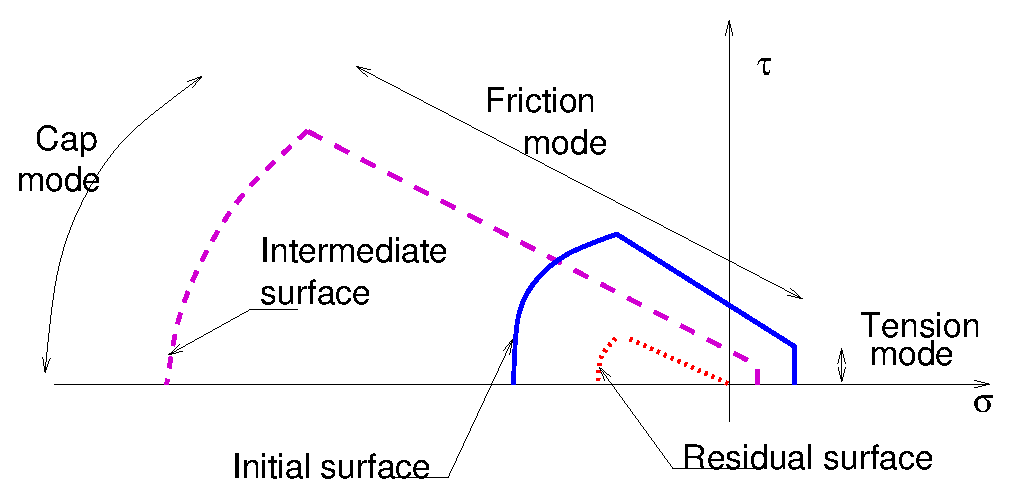
\includegraphics{constmodel.eps}}}
  \caption{Composite yield surface model for masonry}
  \label{compyieldsurffig}
\end{figure}

The approach used in this work is based on idea of concentrating all the damage in the relatively weak joints and, if necessary, in potential tension cracks in the bricks. The joint interface constitutive model should include all important damage mechanisms. Here, the  concept of interface elements is used. An interface element allows to incorporate discontinuities in the displacement field and its behavior is described in terms of a relation between the tractions and relative displacement across the interface. In the present work, these quantities will be denoted as $\sig$, generalized stress, and $\e$, generalized strain. For 2D configuration, $\sig=\{\sigma, \tau\}^T$ and $\e=\{u_n, u_s\}^T$, where $\sigma$ and $\tau$ are the normal and shear components of the traction interface vector and  $n$ and $s$ subscripts distinguish between normal and shear components of displacement vector.
\begin{figure}
  \centerline{\scalebox{0.5}{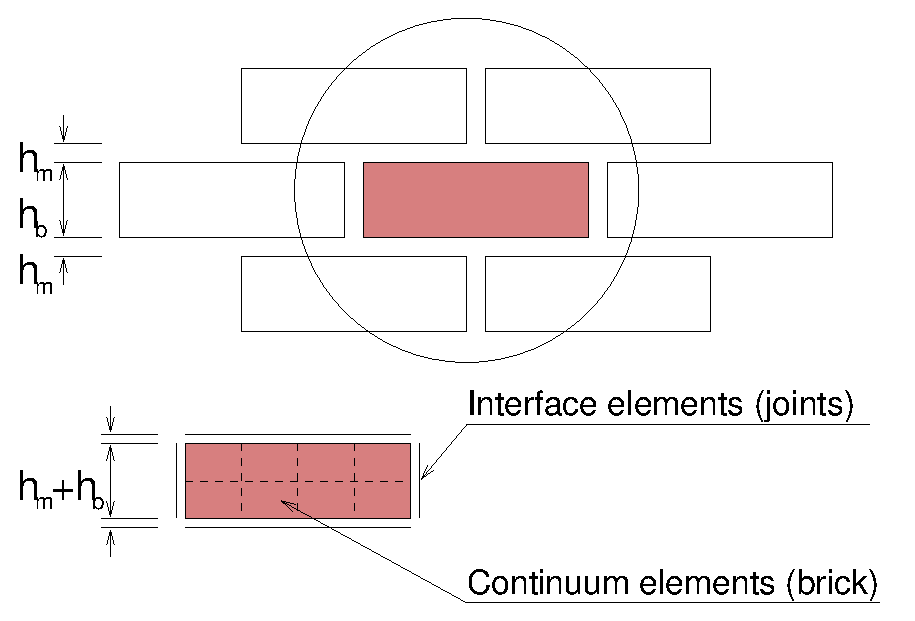
\includegraphics{mmodel.eps}}}
  \caption{Modeling strategy for masonry}
\end{figure}
The elastic response is characterized in terms of elastic constitutive matrix $\mbf{D}$ as
\begin{equation}
  \sig=\mbf{D}\e
\end{equation}
For a 2D configuration $\mbf{D}=diag\{k_n,k_s\}$. The terms of the elastic stiffness matrix can be obtained from the properties of both masonry and joints as
\begin{equation}
  k_n=\del{E_bE_m}{t_m(E_b-E_m)};\;k_s=\del{G_bG_m}{t_m(G_b-G_m)}
\end{equation}
where $E_b$ and $E_m$ are Young's moduli and $G_b$ and $G_m$ shear moduli for brick and mortar. One should note, that there is no contact algorithm assumed between bricks, this means that the overlap of neighboring units will be visible. On the other hand, the interface model includes a compressive cap, where the compressive inelastic behavior of masonry is lumped.
\paragraph{Tension mode}
In the tension mode, the exponential softening law is assumed (see fig.(\ref{tensfig})). The yield function has the following form
\begin{equation}
  f_1(\sig,\kappa_1) = \sigma-f_t(\kappa_1)
\end{equation}
where the yield value $f_t$ is defined as
\begin{equation}
\label{ft}
  f_t=f_{t0}\exp\left(-\del{f_{t0}}{G^I_f}\kappa_1\right)
\end{equation}
\begin{figure}
  \centerline{\scalebox{0.5}{\includegraphics{tension.eps}}}
  \caption{Tensile behavior of proposed model ($f_t=0.2\ \rm{MPa},\ G_f^I=0.018\ \rm{N/mm}$)}
  \label{tensfig}
\end{figure}
The $f_{t0}$ represents tensile strength of joint or interface; and $G^I_f$ is mode-I fracture energy. For the tension mode, the associated flow hypothesis is assumed. 


\paragraph{Shear mode}
For the shear mode a Coulomb friction envelope is used. The yield function has the form
\begin{equation}
  f_2(\sig,\kappa_2) = \vert\tau\vert+\sigma\tan\phi(\kappa_2)-c(\kappa_2)
\end{equation}
According to \cite{Rots} the variations of friction angle $\phi$ and cohesion $c$ are assumed as
\begin{eqnarray}
  \label{c}
  c&=&c_0\exp\left(-\del{c_0}{G^{II}_f}\kappa_2\right)\\
  \tan\phi&=&\tan\phi_0+(\tan\phi_r-\tan\phi_0)\left(\del{c_0-c}{c_0}\right)
\end{eqnarray}
where $c_0$ is initial cohesion of joint, $\phi_0$ initial friction angle, $\phi_r$ residual friction angle, and $G^{II}_f$ fracture energy in mode II failure. A non-associated plastic potential $g_2$ is considered as
\begin{equation}
  g_2=\vert\tau\vert+\sigma\tan\Phi-c
\end{equation}
\begin{figure}
  \centerline{\scalebox{0.5}{\includegraphics{shearconf.eps}}}
  \caption{Shear behavior of proposed model for different confinement levels in MPa ($c_0=0.8\ \rm{MPa},\ \tan\phi_0=1.0,\ \tan\phi_r=0.75,{\rm and}\ G_f^{II}=0.05\ {N/mm}$)}
\end{figure}


\paragraph{Coupling of tension/shear modes}
The tension and Coulomb friction modes are coupled with isotropic softening. This means that the percentage of softening in the cohesion is assumed to be the same as on the tensile strength
\begin{equation}
  \dot\kappa_1=\lambda_1+\del{G^I_f}{G^{II}_f}\del{c_0}{f_{t0}}\lambda_2;\ \ \dot\kappa_2=\del{G^{II}_f}{G^I_f}\del{f_{t0}}{c_0}\lambda_1+\lambda_2
\end{equation}
This follows from (\ref{ft}) and (\ref{c}). However, in the corner region, when both yield surfaces are activated, such approach will lead to a non-acceptable penalty. For this reason a quadratic combination is assumed 
\begin{equation}
  \dot\kappa_1=\sqrt{(\lambda_1)^2+\left(\del{G^I_f}{G^{II}_f}\del{c_0}{f_{t0}}\lambda_2\right)^2};\ \ \dot\kappa_2=\sqrt{\left(\del{G^{II}_f}{G^I_f}\del{f_{t0}}{c_0}\lambda_1\right)^2+(\lambda_2)^2}
\end{equation}

\paragraph{Cap mode}
For the cap mode, an ellipsoid interface model is used. The yield condition is assumed as
\begin{equation}
  f_3(\sig, \kappa_3) = C_{nn}\sigma^2+C_{ss}\tau^2 + C_n\sigma-\bar\sigma^2(\kappa_3)
\end{equation}
where $C_{nn},\ C_{ss}$, and $C_n$ are material model parameters and $\bar\sigma$ is yield value, originally assumed in the following form of hardening/softening law \cite{Rots}
\begin{eqnarray}
  \nonumber
  \bar\sigma_1(\kappa_3)&=&\bar\sigma_i+(\bar\sigma_p-\bar\sigma_i)\sqrt{\del{2\kappa_3}{\kappa_p}-\del{\kappa_3^2}{\kappa_p^2}};\;\;\kappa_3\in(0,\kappa_p)\\
  \label{hs3}
  \bar\sigma_2(\kappa_3)&=&\bar\sigma_p+(\bar\sigma_m-\bar\sigma_p)\left(\del{\kappa_3-\kappa_p}{\kappa_m-\kappa_p}\right)^2;\;\;\kappa_3\in(\kappa_p, \kappa_m)\\
  \nonumber
  \bar\sigma_3(\kappa_3)&=&\bar\sigma_r+(\bar\sigma_m-\bar\sigma_r)\exp\left(m\del{\kappa_3-\kappa_m}{\bar\sigma_m-\bar\sigma_r}\right);\;\;\kappa_3\in(\kappa_m, \infty)
\end{eqnarray}
with $m=2(\bar\sigma_m-\bar\sigma_p)/(\kappa_m-\kappa_p)$. The hardening/softening law (\ref{hs3}) is shown in fig.(\ref{hs3fig}). Note that the curved diagram is a $C^1$ continuous $\sigma-\kappa_3$ relation. The energy under the load-displacement diagram can be related to a ``compressive fracture energy''.
The original hardening law (\ref{hs3}.1) exhibits indefinite slope for $\kappa_3=0$, which can cause the problems with numerical implementation. This has been overcomed by replacing this hardening law with parabolic equation given by
\begin{equation}
  \bar\sigma_1(\kappa_3) = \bar\sigma_i-2*(\bar\sigma_i-\bar\sigma_p)*\del{\kappa_3}{\kappa_p}+(\bar\sigma_i-\bar\sigma_p)\del{\kappa_3}{\kappa_p}
\end{equation}
An associated flow and strain hardening hypothesis are being considered. This yields
\begin{equation}
  \dot\kappa_3=\lambda_3\sqrt{(2C_{nn}\sigma+C_n)*(2C_{nn}\sigma+C_n) + (2C_{ss}\tau)*(2C_{ss}\tau)}
\end{equation}
\begin{figure}
  \centerline{\scalebox{0.5}{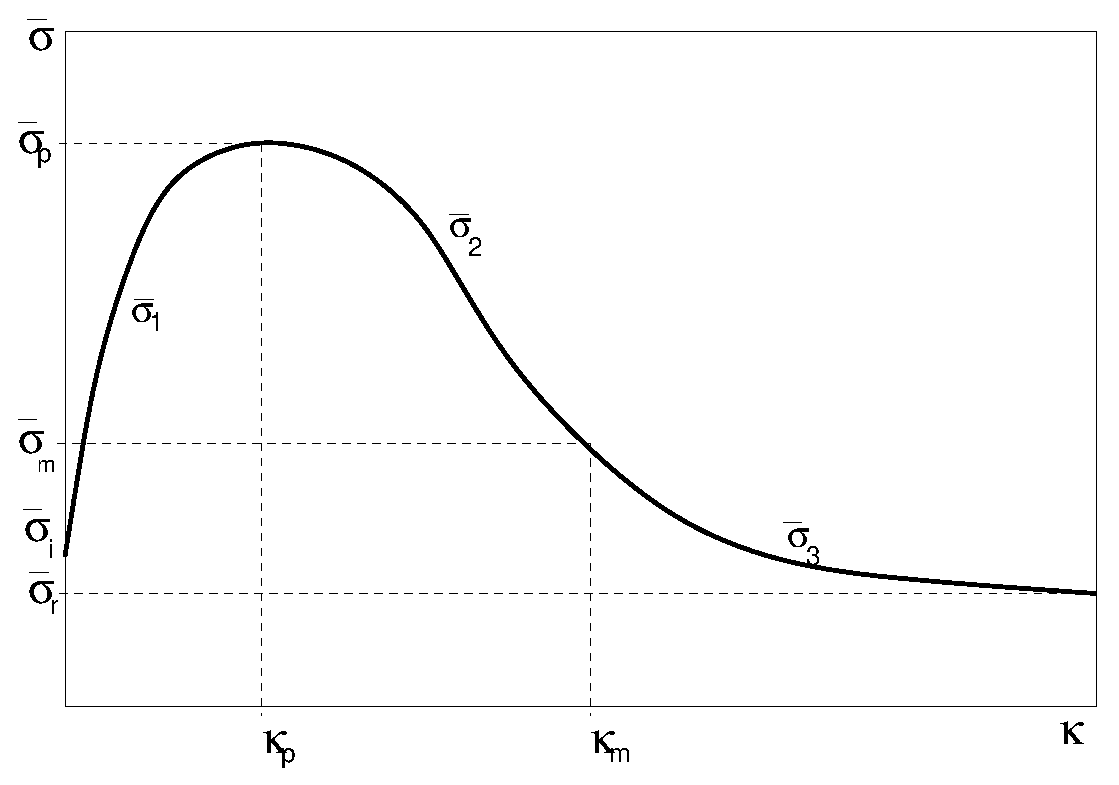
\includegraphics{capmode.eps}}}
\caption{Hardening/softening law for cap mode}
\label{hs3fig}
\end{figure}

The model parameters are summarized in table~\ref{compomasonry1_table}.
There is one algorithmic issue, that follows from the model
formulation. Since the cap mode hardening/softening is not coupled to
hardening/softening of shear and tension modes the it may happen that 
when the cap and shear modes are activated, the return directions
become parallel for both surfaces. This should be avoided by adjusting
the input parameters accordingly (one can modify dilatancy angle, for example). 

\begin{table}[h]                                                                
%\begin{center}                                                                  
\begin{tabular}{|l|p{9cm}|}                                                      
\hline                                                                          
Description & Composite plasticity model for masonry\\
\hline                                                                          
Record Format & \descitem{Masonry02} \elemparam{num}{in} \elemparam{d}{rn} 
\elemparam{ft0}{rn} \elemparam{gfi}{rn}
\elemparam{gfii}{rn}
\elemparam{kn}{rn} \elemparam{ks}{rn} \elemparam{c0}{rn}
\elemparam{tanfi0}{rn} \elemparam{tanfir}{rn} \elemparam{tanpsi}{rn}
\elemparam{si}{rn} \elemparam{sp}{rn} \elemparam{sm}{rn} \elemparam{sr}{rn}
\elemparam{kp}{rn} \elemparam{km}{rn} \elemparam{kr}{rn}
\elemparam{cnn}{rn} \elemparam{css}{rn} \elemparam{cn}{rn}\\
Parameters &- \param{num} material model number\\
&- \param{d} material density\\
&- \param{ft0} tensile strength\\
&- \param{gfi} fracture energy for mode I\\
&- \param{gfii} fracture energy for mode II\\
&- \param{kn} joint elastic property\\
&- \param{ks} joint elastic property\\
&- \param{c0} initial cohesion\\
&- \param{tanfi0} initial friction angle\\
&- \param{tanfir} residual friction angle\\
&- \param{tanpsi} dilatancy\\
&- \param{\{si, sp, sm, sr\}} cap parameters $\{\bar\sigma_i, \bar\sigma_p, \bar\sigma_m, \bar\sigma_r\}$\\
&- \param{\{kp, km,kr\}} cap parameters $\{\kappa_p, \kappa_m, \kappa_r\}$\\
&- \param{cnn},\param{css},\param{cn} cap mode parametrs\\
Supported modes& \_2dInterface\\
\hline
\end{tabular}                                                                   
\caption{Composite model for masonry - summary.}                
\label{compomasonry1_table}                                                         
%\end{center}                                                                    
\end{table}                                                                     


\subsubsection{HMH perfectly plastic material}

Implements a perfectly plastic material. 
HMH plasticity condition with no hardening is used. 
Before plastic condition apply, and during unloading and reloading an
isotropic linear elastic behavior is assumed. Linear elastic behavior
is described using Young modulus and Poisson ratio. Plasticity
condition is described using uniaxial strength. 
The model description and parameters are summarized
in table~\ref{Steel1_table}.

\begin{table}[h]                                                                
%\begin{center}                                                                  
\begin{tabular}{|l|p{9cm}|}                                                      
\hline                                                                          
Description & HMH perfectly plastic material\\
\hline                                                                          
Record Format & \descitem{Steel1} \elemparam{num}{in}
\elemparam{d}{rn} \elemparam{E}{rn} \elemparam{n}{rn}
\elemparam{tAlpha}{rn} \elemparam{Ry}{rn}\\
Parameters &- \param{num} material model number\\
&- \param{d} material density\\
&- \param{E} Young modulus\\
&- \param{n} Poisson ratio\\
&- \param{tAlpha} thermal dilatation coefficient\\
&- \param{Ry} uniaxial strength defining the yield limit\\
Supported modes& 3dMat, PlaneStress, PlaneStrain, 1dMat,
2dPlateLayer, 2dBeamLayer, 3dShellLayer
3dBeam, PlaneStressRot\\
\hline
\end{tabular}                                                                   
\caption{HMH perfectly plastic material - summary.}                
\label{Steel1_table}                                                         
%\end{center}                                                                    
\end{table}                                                                     


\subsubsection{Nonlinear elasto-plastic material model for concrete
plates and shells}
\label{Rer}
Nonlinear elasto-plastic material model with hardening. 
Takes into account uniaxial stress + transverse shear in concrete
layers with transverse stirrups. 
Can be used only for 2d plates and shells with layered cross section 
and together with explicit integration method (stiffness matrix is not
provided). 
The model description and parameters are summarized
in table~\ref{Rer_table}.

\begin{table}[h]                                                                
%\begin{center}                                                                  
\begin{tabular}{|l|p{9cm}|}                                                      
\hline                                                                          
Description & Nonlinear elasto-plastic material model for concrete
plates and shells\\
\hline                                                                          
Record Format & \descitem{Concrete2} \elemparam{num}{in}
\elemparam{d}{rn} \elemparam{E}{rn} \elemparam{n}{rn}
\elemparam{SCCC}{rn} \elemparam{SCCT}{rn} \elemparam{EPP}{rn} \elemparam{EPU}{rn} 
\elemparam{EOPU}{rn} \elemparam{EOPP}{rn} \elemparam{SHEARTOL}{rn}
\elemparam{IS\_PLASTIC\_FLOW}{in} \elemparam{IFAD}{in} \elemparam{STIRR\_E}{rn} \elemparam{STIRR\_Ft}{rn}
\elemparam{STIRR\_A}{rn} \elemparam{STIRR\_TOL}{rn} \elemparam{STIRR\_EREF}{rn}
\elemparam{STIRR\_LAMBDA}{rn}\\ 

Parameters &- \param{num} material model number\\
&- \param{d} material density\\
&- \param{E} Young modulus\\
&- \param{n} Poisson ratio\\
&- \param{SCCC} pressure strength\\
&- \param{SCCT} tension strength\\
&- \param{EPP} threshold effective plastic strain for softening in
compression\\
&- \param{EPU} ultimate eff. plastic strain\\
&- \param{EOPP} threshold volumetric plastic strain for softening in
tension\\
&- \param{EOPU} ultimate volumetric plastic strain\\
&- \param{SHEARTOL} threshold value of the relative shear deformation 
(psi**2/eef) at which shear is considered in layers. 
For lower relative shear deformations the transverse shear remains elastic decoupled from bending. default value
SHEARTOL = 0.01\\
&- \param{IS\_PLASTIC\_FLOW} indicates that plastic flow (not
deformation theory) is used in pressure\\
&- \param{IFAD} State variables will not be updated, otherwise update state variables\\
&- \param{STIRR\_E} Young modulus of stirrups\\
&- \param{STIRR\_R} stirrups uniaxial strength = elastic limit\\
&- \param{STIRR\_A} stirrups area/unit length (beam) or /unit area (shell)\\
&- \param{STIRR\_TOL} stirrups tolerance of equilibrium in the z direction (=0 no iteration)\\
&- \param{STIRR\_EREF} stirrups reference strain rate for Peryzna's
material\\
&- \param{STIRR\_LAMBDA} coefficient for that material (stirrups)\\
&- \param{SHTIRR\_H} isotropic hardening factor for stirrups\\
Supported modes& 3dShellLayer, 2dPlateLayer\\
\hline
\end{tabular}                                                                   
\caption{Nonlinear elasto-plastic material model for concrete - summary.}                
\label{Rer_table}                                                         
%\end{center}                                                                    
\end{table}                                                                     

\subsubsection{J2 plasticity material model with hardening}

\subsection{Material models for tensile failure}
\subsubsection{Nonlinear elasto-plastic material model for concrete
plates and shells}
The description can be found is section~\ref{Rer}.

\subsubsection{Smeared rotating crack model}
\label{rcm}
Implementation of smeared rotating crack model. 
Virgin material is modeled as isotropic linear elastic material
(described by Young modulus and Poisson
ratio). The onset of cracking begins, when principal stress reaches
tensile strength. 
Further behavior is then determined by softening law, 
governed by principle of preserving of fracture
energy $G_f$. For large elements, the tension strength can be
artificially reduced
to preserve fracture energy. Multiple cracks are allowed. 
The elastic unloading and reloading is assumed. 
In compression regime, this model correspond to isotropic linear elastic material.
The model description and parameters are summarized
in table~\ref{rcm_table}.

\begin{table}[h]                                                                
%\begin{center}                                                                  
\begin{tabular}{|l|p{9cm}|}                                                      
\hline                                                                          
Description & Rotating crack model for concrete\\
\hline                                                                          
Record Format & \descitem{Concrete3} \elemparam{d}{rn} \elemparam{E}{rn}
\elemparam{n}{rn} \elemparam{Gf}{rn} \elemparam{Ft}{rn} \elemparam{exp\_soft}{in} \elemparam{tAlpha}{rn} \\
Parameters &- \param{num} material model number\\
&- \param{d} material density\\
&- \param{E} Young modulus\\
&- \param{n} Poisson ratio\\
&- \param{Gf} fracture energy\\
&- \param{Ft} tension strength\\
&- \param{exp\_soft} determines the type of softening, if nonzero
exponential softening is used, linear otherwise\\
&- \param{tAlpha} thermal dilatation coefficient\\
Supported modes& 3dMat, PlaneStress, PlaneStrain, 1dMat,
2dPlateLayer, 2dBeamLayer, 3dShellLayer\\
\hline
\end{tabular}                                                                   
\caption{Rotating crack model for concrete - summary.}                
\label{rcm_table}                                                         
%\end{center}                                                                    
\end{table}                                                                     



\subsubsection{Smeared rotating crack model with transition to scalar
damage - linear softening}
\label{rcsd}
Implementation of smeared rotating crack model with transition to
scalar damage with linear softening law. 
Improves the classical rotating model (see
section~\ref{rcm}) by introducing the transition to scalar damage
model in  later stages of tension softening. 

Traditional smeared-crack models for concrete fracture are known to suffer by stress locking (meaning here spurious stress transfer across widely opening cracks),
mesh-induced directional bias, and possible instability at late stages of the loading process.
The combined model keeps the anisotropic character of the rotating
crack but it does not transfer spurious stresses across
widely open cracks.
The new model with transition to
scalar damage (RC-SD) keeps the anisotropic character of the RCM but
it does not transfer spurious stresses across widely open cracks.

Virgin material is modeled as isotropic linear elastic material
(described by Young modulus and Poisson
ratio). The onset of cracking begins, when principal stress reaches
tensile strength. 
Further behavior is then determined by {\bf linear} softening law, 
governed by principle of preserving of fracture
energy $G_f$. For large elements, the tension strength can be
artificially reduced
to preserve fracture energy.  The transition to scalar damage model
takes place, when the softening stress reaches the specified limit.
Multiple cracks are allowed. 
The elastic unloading and reloading is assumed. 
In compression regime, this model correspond to isotropic linear elastic material.
The model description and parameters are summarized
in table~\ref{rcsd_table}.

\begin{table}[h]                                                                
%\begin{center}                                                                  
\begin{tabular}{|l|p{9cm}|}                                                      
\hline                                                                          
Description & RC-SD model for concrete\\
\hline                                                                          
Record Format & \descitem{RCSD} \elemparam{d}{rn} \elemparam{E}{rn}
\elemparam{n}{rn} \elemparam{Gf}{rn} \elemparam{Ft}{rn} \elemparam{sdtransitioncoeff}{rn} \elemparam{tAlpha}{rn} \\
Parameters &- \param{num} material model number\\
&- \param{d} material density\\
&- \param{E} Young modulus\\
&- \param{n} Poisson ratio\\
&- \param{Gf} fracture energy\\
&- \param{Ft} tension strength\\
&- \param{sdtransitioncoeff} determines the transition from RC to SD
model. Transition takes plase when ratio of current softening
stress to tension strength is less than  \param{sdtransitioncoeff} value\\
&- \param{tAlpha} thermal dilatation coefficient\\
Supported modes& 3dMat, PlaneStress, PlaneStrain, 1dMat,
2dPlateLayer, 2dBeamLayer, 3dShellLayer\\
\hline
\end{tabular}                                                                   
\caption{RC-SD model for  concrete - summary.}                
\label{rcsd_table}                                                         
%\end{center}                                                                    
\end{table}                                                                     

\subsubsection{Smeared rotating crack model with transition to scalar
damage - exponential softening}
\label{rcsde}
Implementation of smeared rotating crack model with transition to
scalar damage with exponential softening law. 
The description and model summary (table~\ref{rcsde_table}) are the
same as for the RC-SD model with linear softening law (see section~\ref{rcsd}).
\begin{table}[h]                                                                
%\begin{center}                                                                  
\begin{tabular}{|l|p{9cm}|}                                                      
\hline                                                                          
Description & RC-SD model for concrete with exponential softening law\\
\hline                                                                          
Record Format & \descitem{RCSDE} \elemparam{d}{rn} \elemparam{E}{rn}
\elemparam{n}{rn} \elemparam{Gf}{rn} \elemparam{Ft}{rn} \elemparam{sdtransitioncoeff}{rn} \elemparam{tAlpha}{rn} \\
\hline
\end{tabular}                                                                   
\caption{RC-SD model for  concrete - summary.}                
\label{rcsde_table}                                                         
%\end{center}                                                                    
\end{table}                                                                     

\subsubsection{Nonlocal Smeared rotating crack model with transition to scalar damage}
\label{rcsdnl}
Implementation of nonlocal version of smeared rotating crack model with transition to
scalar damage. 
Improves the classical rotating model (see
section~\ref{rcm}) by introducing the transition to scalar damage
model in  later stages of tension softening. 
The improved RC-SD (see section~\ref{rcsd}) is further extended to a
nonlocal formulation, which not only acts as a powerful localization
limiter but also alleviates mesh-induced directional bias. A special
type of material instability arising due to negative shear stiffness
terms in the rotating crack model is resolved by switching to SD mode. A bell shaped nonlocal
averaging function is used.

Virgin material is modeled as isotropic linear elastic material
(described by Young modulus and Poisson
ratio). The onset of cracking begins, when principal stress reaches
tensile strength. 
Further behavior is then determined by {\bf exponential} softening law.

The transition to scalar damage model
takes place, when the softening stress reaches the specified limit or
when the loss of material stability due to negative shear stiffness
terms that may arise in the standard RCM formulation, which takes
place when the ratio of minimal shear coefficient in stiffness to
bulk material shear modulus reaches the limit.

Multiple cracks are allowed. 
The elastic unloading and reloading is assumed. 
In compression regime, this model correspond to isotropic linear elastic material.
The model description and parameters are summarized
in table~\ref{rcsdnl_table}.

\begin{table}[h]                                                                
%\begin{center}                                                                  
\begin{tabular}{|l|p{9cm}|}                                                      
\hline                                                                          
Description & RC-SD-NL model for concrete\\
\hline                                                                          
Record Format & \descitem{RCSDNL} \elemparam{d}{rn} \elemparam{E}{rn}
\elemparam{n}{rn}  \elemparam{Ft}{rn}
\elemparam{sdtransitioncoeff}{rn} \elemparam{sdtransitioncoeff2}{rn}
\elemparam{r}{rn} \elemparam{tAlpha}{rn} \\
Parameters &- \param{num} material model number\\
&- \param{d} material density\\
&- \param{E} Young modulus\\
&- \param{n} Poisson ratio\\
&- \param{ef} deformation corresponding to fully open crack\\
&- \param{Ft} tension strength\\
&- \param{sdtransitioncoeff} determines the transition from RC to SD
model. Transition takes place when ratio of current softening
stress to tension strength is less than  \param{sdtransitioncoeff} value\\
&- \param{sdtransitioncoeff2} determines the transition from RC to SD
model. Transition takes place when ratio of current minimal shear
stiffness term to virgin shear modulus is less than  \param{sdtransitioncoeff2} value\\
&- \param{r} parameter specifying the width of nonlocal averaging zone\\
&- \param{tAlpha} thermal dilatation coefficient\\
&- \param{regionMap} map indicating the regions (currently region is
characterized by cross section number) to skip for nonlocal
avaraging. The elements and corresponding IP are not taken into
account in nonlocal averaging process if corresponding regionMap
value is nonzero.\\
Supported modes& 3dMat, PlaneStress, PlaneStrain, 1dMat,
2dPlateLayer, 2dBeamLayer, 3dShellLayer\\
\hline
\end{tabular}                                                                   
\caption{RC-SD-NL model for  concrete - summary.}                
\label{rcsdnl_table}                                                         
%\end{center}                                                                    
\end{table}                                                                     


\subsubsection{Isotropic damage model in tension}
This isotropic damage model assumes that the stiffness degradation is
isotropic, i.e., stiffness moduli corresponding to different
directions decrease proportionally and independently of direction of
loading. The damaged stiffness tensor is expressed as
$\mbf{D}=(1-\omega)\mbf{D}^e$.
Damage evolution law is postulated in an explicit form, relating
damage parameter and scalar measure of largest reached equivalent strain level in
material e, taking into account the principle of preserving of fracture
energy $G_f$. The equivalent strain, i.e., a scalar measure of the
strain level is defined as norm from positive principal strains.
The model description and parameters are summarized
in table~\ref{id_table}. The material uses crack-band approach to dissipate the 
correct annount of fracture energy by adjusting locally material parameters. 
There is a limit on element size, which can be expressed as
$$
e0 \le ef/l_e
$$
where $l_e$ is element length in the direction normal to crack plane, e0 is max effective strain at peak load, 
and ef is crack opening (not strain) when tension stress vanishes.
This condition prevents a local snap-back of stress-strain diagram, 
which will otherwise occur to preserve correct amount of dissipated energy for large elements. 


\begin{table}[h]                                                                
%\begin{center}                                                                  
\begin{tabular}{|l|p{9cm}|}                                                      
\hline                                                                          
Description & Isotropic damage model  for concrete in tension\\
\hline                                                                          
Record Format & \descitem{idm1} \elemparam{d}{rn} \elemparam{E}{rn}
\elemparam{n}{rn}  \elemparam{e0}{rn}
\elemparam{ef}{rn} \elemparam{tAlpha}{rn} \elemparam{equivstraintype}{in}\\
Parameters &- \param{num} material model number\\
&- \param{d} material density\\
&- \param{E} Young modulus\\
&- \param{n} Poisson ratio\\
&- \param{ef} crack opening (not strain) when tension stress vanishes\\
&- \param{e0} max effective strain at peak\\
&- \param{tAlpha} thermal dilatation coefficient\\
&- \param{equivstraintype} Allows to choose from different definitions
of equivalent strain, which is a scalar measure of the strain
level. The supported values are: 
\begin{itemize}
\item[0-] Mazar's definition of equivalent
strain (default one)
$\tilde\varepsilon=\sqrt{\displaystyle{\sum_{I=1}^{3}}<\varepsilon_I>^2}$,
where $<\varepsilon_I>$ are positive parts of principal values of
strain tensor,
\item[1-] corresponds to Rankine criterion of maximum principal stress and is based on
the positive part of the  effective stress
($\tilde\varepsilon={{1}\over{E}}\sqrt{\displaystyle{\sum_{I=1}^{3}}<\bar\sigma_I>^2}$), where
$<\bar\sigma_I>$ are the positive parts of principal values of the
effective stress tensor $\bar\sigma = \mbf{D}_e:\varepsilon$, 
\item[2-] equivalent
strain defined as energy norm normalized by Young's modulus to obtain
strain-like quantity
($\tilde\varepsilon=\sqrt{{\varepsilon:\mbf{D}:\varepsilon}\over{E}}$)
\end{itemize}\\
Supported modes& 3dMat, PlaneStress, PlaneStrain, 1dMat\\
Features & Adaptivity support\\
\hline
\end{tabular}                                                                   
\caption{Isotropic Damage model in tension - summary.}                
\label{id_table}                                                         
%\end{center}                                                                    
\end{table}                                                                     


\subsubsection{Nonlocal isotropic damage model in tension}
Nonlocal version of isotropic damage model in tension. 
The nonlocal averaging acts as a powerful localization
limiter. The bell-shaped nonlocal averaging function is used.
The model description and parameters are summarized
in table~\ref{idnl_table}.


\begin{table}[h]                                                                
%\begin{center}                                                                  
\begin{tabular}{|l|p{9cm}|}                                                      
\hline                                                                          
Description & Nonlocal isotropic damage model  for concrete in tension\\
\hline                                                                          
Record Format & \descitem{idmnl1} \elemparam{d}{rn} \elemparam{E}{rn}
\elemparam{n}{rn}  \elemparam{e0}{rn}
\elemparam{ef}{rn} \elemparam{tAlpha}{rn} \\
Parameters &- \param{num} material model number\\
&- \param{d} material density\\
&- \param{E} Young modulus\\
&- \param{n} Poisson ratio\\
&- \param{ef} $\varepsilon_f$ is a model parameter that controls
the post-peak slope (the tangent modulus just after the peak is
$E_t=-f_t/(\varepsilon_f-\varepsilon_0)$)\\
&- \param{e0} max effective strain at peak\\
&- \param{r} nonlocal interaction radius\\
&- \param{tAlpha} thermal dilatation coefficient\\
&- \param{regionMap} map indicating the regions (currently region is
characterized by cross section number) to skip for nonlocal
avaraging. The elements and corresponding IP are not taken into
account in nonlocal averaging process if corresponding regionMap
value is nonzero.\\
&- \param{equivstraintype} Allows to choose from different definitions
of equivalent strain, which is a scalar measure of the strain
level. For the description, see table \ref{id_table}.\\
Supported modes& 3dMat, PlaneStress, PlaneStrain, 1dMat\\
Features & Adaptivity support\\
\hline
\end{tabular}                                                                   
\caption{Nonlocal isotropic Damage model in tension - summary.}                
\label{idnl_table}                                                         
%\end{center}                                                                    
\end{table}                                                                     

%------------------------------------------------------------------
\subsubsection{MDM - Anisotropic damage model}
%------------------------------------------------------------------

\paragraph{Local formulation}

The concept of isotropic damage is appropriate for materials weakened
by voids, but if the physical source of damage is the initiation and
propagation of microcracks, isotropic stiffness degradation 
can be considered only as a first rough
approximation. More refined damage models take into account the highly
oriented nature of cracking, which is reflected by the anisotropic
character of the damaged stiffness or compliance matrices.

A number of anisotropic damage formulations have been proposed
in the literature. Here we use a model outlined by M. Jir\'{a}sek
in \cite{mdm}, which is based on the principle of energy
equivalence and on the construction of the inverse integrity
tensor by integration of a scalar over all spatial directions. 
Since the model uses certain concepts from the
microplane theory, it is called the microplane-based damage model (MDM).

The general structure of the MDM 
model is schematically shown in Fig.\ \ref{ff4}
and the basic equations are summarized in Table \ref{tab2}.
Here, $\veps$ and $\vsig$ are the (nominal) second-order 
strain and stress tensors
with components $\eps_{ij}$ and $\sigma_{ij}$; $\ve$ and $\vs$
are first-order strain and stress tensors with components $e_i$
and $s_i$, which characterize the strain and stress on ``microplanes''
of different orientations given by a unit vector $\mbf{n}$
with components $n_i$;
$\psi$ is a dimensionless compliance parameter 
that is a scalar but can have different values for different 
directions $\mbf{n}$;
the symbol $\delta$ denotes a virtual quantity; and a sumperimposed
tilde denotes an effective quantity, which is supposed to characterize the
state of the intact material between defects such as microcracks or voids.

\begin{table}[h]
\caption{Basic equations of microplane-based anisotropic damage model}
\label{tab2}
\begin{center}
\begin{tabular}{|c|c|c|}
\hline
&&\\
$\vet=\vepst\cdot\mbf{n}$ 
&
$\vst = \psi\vs$ 
&
$\vs=\vsig\cdot\mbf{n}$ 
\\[5mm]
$\vsigt:\dvepst = \displaystyle\frac{3}{2\pi} \int_{\Omega}\vst\cdot\dvet\;\mbox{d}\Omega$
& 
$\dvs\cdot\ve=d\vst\cdot\vet$ 
&
$\dvsig:\veps = \displaystyle\frac{3}{2\pi} \int_{\Omega}\dvs\cdot\ve\dO$
\\[5mm]
$\vsigt = \displaystyle\frac{3}{2\pi}\int_\Omega (\vst\otimes\mbf{n})\sym\dO$
&
$\ve=\psi\vet$
&
$\veps = \displaystyle\frac{3}{2\pi}\int_\Omega (\ve\otimes\mbf{n})\sym\dO$
\\[5mm]
\hline
\end{tabular}
\end{center}
\end{table}

\begin{figure}
%\begin{center}
%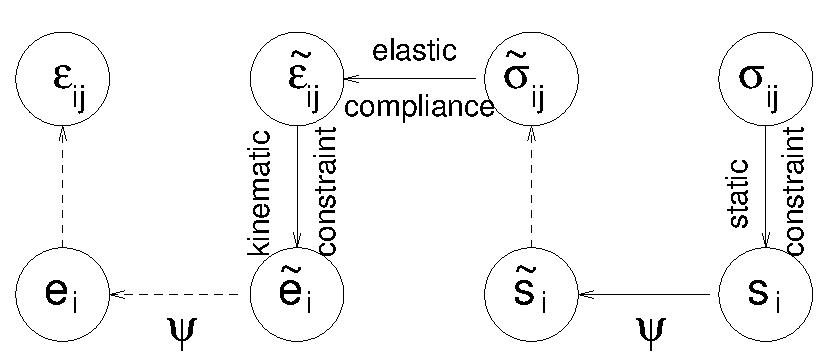
\includegraphics[width=10cm]{dm_comp.eps}
\centerline{\scalebox{0.8}{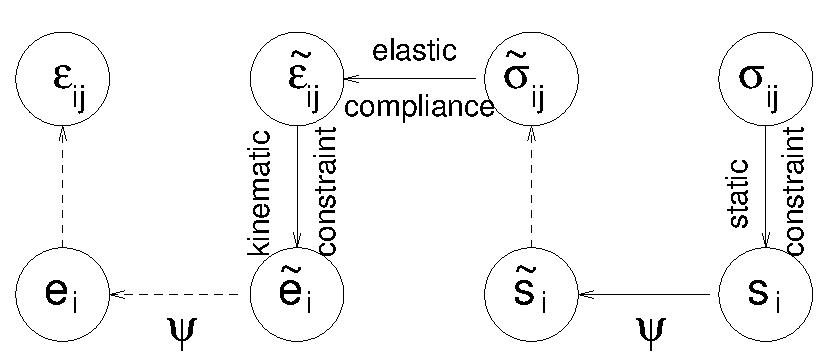
\includegraphics{dm_comp.eps}}}
%\end{center}
\caption{Structure of microplane-based anisotropic damage model}
\label{ff4}
\end{figure}

Combining the basic equations, it is possible to show that the 
components of the damaged
material compliance tensor are given by 
\begin{equation}
\label{damcom}
C_{ijkl}=M_{pqij}M_{rskl}C^e_{pqrs}
\end{equation}
where $C^e_{pqrs}$ are the components of the elastic material compliance tensor,
\begin{equation}
\label{ee27}
M_{ijkl} = \quarter\left(
\psi_{ik}\delta_{jl}+\psi_{il}\delta_{jk}+\psi_{jk}\delta_{il}+\psi_{jl}\delta_{ik}\right)
\end{equation}
are the components of the so-called damage effect tensor, and
\begin{equation}
\label{ee24}
\psi_{ij} = \frac{3}{2\pi}\int_\Omega \psi\, n_i n_j \dO
\end{equation}
are the components of the second-order inverse integrity tensor.
The integration domain $\Omega$ is the unit hemisphere.
In practice, the integral over the unit hemisphere is evaluated by
summing the contribution from a finite number of directions, according
to one of the numerical integration schemes that are used by microplane
models. 

The scalar variable $\psi$ characterizes the relative compliance
in the direction given by the vector $\mbf{n}$. 
If $\psi$ is the same in all directions,
the inverse integrity tensor  evaluated from (\ref{ee24})
is equal to the unit second-order tensor (Kronecker delta) multiplied
by $\psi$, the damage effect tensor evaluated from (\ref{ee27})
is equal to the symmetric fourth-order unit tensor multiplied
by $\psi$, 
and the damaged
material compliance tensor evaluated from (\ref{damcom}) is the
elastic compliance tensor multiplied by $\psi^2$. The factor multiplying
the elastic compliance tensor in the 
isotropic damage model is $1/(1-\omega)$, and so $\psi$ corresponds
to  $1/\sqrt{1-\omega}$. In the initial undamaged state,
$\psi=1$ in all directions.  The evolution of $\psi$
is governed by the history of the projected strain components.
In the simplest case, $\psi$ is driven by the normal strain
$e_N=\eps_{ij}n_in_j$. Analogy with the isotropic damage model
leads to the damage law
\begin{equation}
\psi=f(\kappa)
\end{equation}
and loading-unloading conditions
\begin{equation}
g(e_N,\kappa)\equiv e_N-\kappa\le 0, \hskip 10mm
\dot{\kappa}\ge 0, \hskip 10mm
\dot{\kappa}g(e_N,\kappa)=0
\end{equation}
in which $\kappa$ is a history variable that represents the maximum
level of normal strain in the given direction ever reached in the
previous history of the material. An appropriate modification
of the exponential softening
law leads to the damage law
\begin{equation}
\label{expsoft2}
f(\kappa)=\left\{
\begin{array}{ll}
1 & \mbox{ if } \kappa\le e_0
\\
\sqrt{\frac{\kappa}{e_0}\exp\left(\frac{\kappa-e_0}{e_f-e_0}\right)} 
& \mbox{ if } \kappa>e_0
\end{array}
\right.
\end{equation}
where $e_0$ is a parameter controlling the elastic limit, and $e_f>e_0$
is another parameter controlling ductility. 
Note that softening in a limited number of directions does not necessarily
lead to softening on the macroscopic level, because the response
in the other directions remains elastic. Therefore, $e_0$ corresponds
to the elastic limit but not to the state at peak stress.

If the MDM model is used in its basic form described above, 
the compressive strength turns out to depend on the Poisson ratio and,
in applications to concrete, its value is too low compared to the
tensile strength. The model is designed primarily for tensile-dominated
failure, so the low compressive strength 
is not considered as a major drawback. Still, it
is desirable to introduce a modification that would prevent spurious
compressive failure in problems where moderate compressive stresses
appear. The desired effect is achieved by redefining the projected
strain $e_N$ as
\begin{equation}
\label{ee37}
e_N =  \frac{\eps_{ij}n_in_j}{1-\displaystyle\frac{m}{Ee_0}\sigma_{kk}}
\end{equation}
where $m$ is a nonnegative parameter that controls the sensitivity to the
mean stress, $\sigma_{kk}$ is the trace of the stress tensor,
and the normalizing factor 
$Ee_0$ is introduced in order to render the parameter
$m$ dimensionless. 
Under compressive stress states (characterized by $\sigma_{kk}<0$), 
the denominator in (\ref{ee37}) is larger than 1, and the projected strain
is reduced, which also leads to a reduction of damage. 
A typical recommended value of parameter $m$ is 0.05. 

\paragraph{Nonlocal formulation}

Nonlocal formulation of the MDM model is based on the averaging of
the inverse integrity tensor. This roughly corresponds to the nonlocal
isotropic damage model with averaging of the compliance variable 
$\gamma=\omega/(1-\omega)$, which does not cause any spurious locking effects.
In equation (\ref{ee27}) for the evaluation of the damage effect tensor,
the inverse integrity tensor is replaced by its weighted average with
components
\begin{equation}
\label{psinl1}
\bar{\psi}_{ij}(\vx)=\int_V \alpha(\vx,\vxi)\psi_{ij}(\vxi)\mbox{d}\vxi
\end{equation}

By fitting a wide range of numerical results, it has been found that
the parameters of the nonlocal MDM model can be estimated from the
measurable material properties using the formulas
\begin{eqnarray}
\lambda_f&=&\frac{EG_f}{Rf_t^2}
\\
\lambda&=&\frac{\lambda_f}{1.47-0.0014\lambda_f}
\\
e_0&=&\frac{f_t}{(1-m)E(1.56+0.006\lambda)}
\\
e_f&=&e_0[1+(1-m)\lambda]
\end{eqnarray}
where $E$ is Young's modulus, $G_f$ is the fracture energy, $f_t$
is the uniaxial tensile strength, 
$m$ is the compressive correction factor, typically chosen
as $m=0.05$, and $R$ is the radius of nonlocal interaction reflecting the
internal length of the material.
\paragraph{Input Record}
The model description and parameters are summarized
in table~\ref{mdm_table}.

\begin{table}[h]                                                                
%\begin{center}                                                                  
\begin{tabular}{|l|p{9cm}|}                                                      
\hline                                                                          
Description & MDM Anisotropic damage model\\
\hline                        
& Common parameters\\
Record Format & \descitem{mdm} \elemparam{d}{rn} \elemparam{nmp}{ins} \elemparam{talpha}{rn}
\elemparam{parmd}{rn}  \elemparam{nonloc}{in}
\elemparam{formulation}{in} \elemparam{mode}{in}\\
Parameters & -\param{num} material model number\\
& - \param{D} material density\\
& - \param{nmp} number of microplanes used for hemisphere integration,
supported values are 21,28, and 61\\
& - \param{talpha}  thermal dillatation coeff\\
& - \param{parmd} \\
& - \param{nonloc} \\
& - \param{formulation}\\
& - \param{mode}\\
\hline
Nonlocal variant I&\\
Additional params &\elemparam{r}{rn} \elemparam{efp}{rn}
\elemparam{ep}{rn} \\
& -\param{r} nonlocal interaction radius\\
& -\param{efp} $\varepsilon_fp$ is a model parameter that controls
the post-peak slope $\varepsilon_fp$ =$\varepsilon_f-\varepsilon_0$,
where $\varepsilon_f$ is strain at zero stress level.\\
& -\param{ep} max effective strain at peak $\varepsilon_0$\\
\hline
Nonlocal variant II&\\
Additional params &\elemparam{r}{rn} \elemparam{gf}{rn}
\elemparam{ft}{rn}\\
& -\param{r} nonlocal intraction radius\\
& -\param{gf} fracture energy\\
& -\param{ft} tensile strength\\
\hline
Local variant I&\\
Additional params &\elemparam{efp}{rn} \elemparam{ep}{rn}\\
& -\param{efp} $\varepsilon_fp$ is a model parameter that controls
the post-peak slope $\varepsilon_fp$ =$\varepsilon_f-\varepsilon_0$,
where $\varepsilon_f$ is strain at zero stress level.\\
& -\param{ep} max effective strain at peak $\varepsilon_0$\\
\hline
Local variant II&\\
Additional params &\elemparam{gf}{rn} \elemparam{ep}{rn}\\
& -\param{gf} fracture energy\\
& -\param{ep} max effective strain at peak $\varepsilon_0$\\
\hline
Supported modes& 3dMat, PlaneStress\\
Features & Adaptivity support\\
\hline
\end{tabular}                                                                   
\caption{MDM model - summary.}                
\label{mdm_table}                                                         
%\end{center}                                                                    
\end{table}                                                                     



\subsection{Material models specific to concrete}
\subsubsection{Mazars damage model for concrete}
This isotropic damage model assumes that the stiffness degradation is
isotropic, i.e., stiffness moduli corresponding to different
directions decrease proportionally and independently of direction of
loading. 	
It introduces two damage parameters $\omega_t$ and $\omega_c$ that
are computed from the same equivalent strain using two different damage functions
$g_t$ and $g_c$. The $g_t$ is identified from the uniaxial tension tests, while
$g_c$ from compressive test. The damage parameter for general stress states 
$\omega$ is obtained as a linear combination of $\omega_t$ and $\omega_c$:
$\omega=\alpha_t g_t + \alpha_c g_c$, where the coefficients
$\alpha_t$ and $\alpha_c$ take into account the character of the
stress state.
The damaged stiffness tensor is expressed as
$\mbf{D}=(1-\omega)\mbf{D}^e$.
Damage evolution law is postulated in an explicit form, relating
damage parameter and scalar measure of largest reached strain level in
material, taking into account the principle of preserving of fracture
energy $G_f$. The equivalent strain, i.e., a scalar measure of the
strain level is defined as norm from positive principal strains.
The model description and parameters are summarized
in table~\ref{maz_table}.


\begin{table}[h]                                                                
%\begin{center}                                                                  
\begin{tabular}{|l|p{9cm}|}                                                      
\hline                                                                          
Description & Mazars damage model for concrete\\
\hline                                                                          
Record Format & \descitem{mazarsmodel} \elemparam{d}{rn} \elemparam{E}{rn}
\elemparam{n}{rn}  \elemparam{e0}{rn}
\elemparam{ac}{rn} \elemparam{bc}{rn} \elemparam{beta}{rn}
\elemparam{hreft}{rn} \elemparam{hrefc}{rn} 
\elemparam{version}{in} \elemparam{at}{rn} \optelemparam{bt}{rn}
\elemparam{tAlpha}{rn} \\
Parameters &- \param{num} material model number\\
&- \param{d} material density\\
&- \param{E} Young modulus\\
&- \param{n} Poisson ratio\\
&- \param{tAlpha} thermal dilatation coefficient\\
&- \param{version} Model variant. if 0 specified, the original form 
$g_t   = 1.0-(1.0-A_t)*\varepsilon_0/\kappa - A_t*\exp(-B_t*(\kappa-\varepsilon_0));
$ of
tension damage evolution law is used, if equal 1, the modified law
used which asymptotically tends to zero 
$g_t = 1.0-(\varepsilon_0/\kappa)*\exp((\varepsilon_0-\kappa)/A_t)$\\
&- \param{ac},\param{bc} material parameters related to the shape of
uniaxial compression curve (A sample set used by Saouridis is $A_c =
1.34, B_c = 2537$\\
&- \param{at}, \optparam{bt} material parameters related to the shape of
uniaxial tension curve. Meaning dependent on \param{version}
parameter.\\
&- \param{beta} coefficient reducing the effect of damage under
response under shear. Default value set to 1.06\\
&- \param{hreft}, \param{hrefc} reference characteristic lengths for
tension and compression. The material parameters are specified for
element with these characteristic lengths. The current element then
will have the same COD (Crack Opening Displacement) as reference one.\\
Supported modes& 3dMat, PlaneStress, PlaneStrain, 1dMat\\
\hline
\end{tabular}                                                                   
\caption{Mazars Damage model  - summary.}                
\label{maz_table}                                                         
%\end{center}                                                                    
\end{table}                                                                     

\subsubsection{Nonlocal Mazars damage model for concrete}
The nonlocal variant of Mazars damage model for concrete.
Model based on nonlocal averaging of equivalent strain.
The nonlocal averaging acts as a powerful localization
limiter. The bell-shaped nonlocal averaging function is used.
The model description and parameters are summarized
in table~\ref{maznl_table}.

\begin{table}[h]                                                                
%\begin{center}                                                                  
\begin{tabular}{|l|p{9cm}|}                                                      
\hline                                                                          
Description & Nonlocal Mazars damage model for concrete\\
\hline                                                                          
Record Format & \descitem{mazarsmodelnl} \elemparam{r}{rn} \elemparam{E}{rn}
\elemparam{n}{rn}  \elemparam{e0}{rn}
\elemparam{ac}{rn} \elemparam{bc}{rn} \elemparam{beta}{rn}
\elemparam{version}{in} \elemparam{at}{rn} \optelemparam{bt}{rn} \elemparam{r}{rn}
\elemparam{tAlpha}{rn} \\
Parameters &- \param{num} material model number\\
&- \param{d} material density\\
&- \param{E} Young modulus\\
&- \param{n} Poisson ratio\\
&- \param{tAlpha} thermal dilatation coefficient\\
&- \param{version} Model variant. if 0 specified, the original form 
$g_t   = 1.0-(1.0-A_t)*\varepsilon_0/\kappa - A_t*\exp(-B_t*(\kappa-\varepsilon_0));
$ of
tension damage evolution law is used, if equal 1, the modified law
used which asymptotically tends to zero 
$g_t = 1.0-(\varepsilon_0/\kappa)*\exp((\varepsilon_0-\kappa)/A_t)$\\
&- \param{ac},\param{bc} material parameters related to the shape of
uniaxial compression curve (A sample set used by Saouridis is $A_c =
1.34, B_c = 2537$\\
&- \param{at}, \optparam{bt} material parameters related to the shape of
uniaxial tension curve. Meaning dependent on \param{version}
parameter.\\
&- \param{beta} coefficient reducing the effect of damage under
response under shear. Default value set to 1.06\\
&- \param{r} parameter specifying the width of nonlocal averaging zone\\
Supported modes& 3dMat, PlaneStress, PlaneStrain, 1dMat\\
\hline
\end{tabular}                                                                   
\caption{Nonlocal Mazars Damage model  - summary.}                
\label{maznl_table}                                                         
%\end{center}                                                                    
\end{table}                                                                     



\subsubsection{CebFip78 model for concrete aging}
Implementation of CebFip78 material model for concrete aging.
The model description and parameters are summarized
in table~\ref{cebfip_table}.

\begin{table}[h]                                                                
%\begin{center}                                                                  
\begin{tabular}{|l|p{9cm}|}                                                      
\hline                                                                          
Description & CebFip78 Material model  for concrete aging\\
\hline                                                                          
Record Format & \descitem{CebFip78}  \elemparam{n}{rn}
\elemparam{relMatAge}{rn} \elemparam{E28}{rn} \elemparam{fibf}{rn} \elemparam{kap\_a}{rn}
\elemparam{kap\_c}{rn} \elemparam{kap\_tt}{rn} \elemparam{u}{rn}\\ 
Parameters &- \param{num} material model number\\
&- \param{E28} Young modulus at age of 28 days [MPa]\\
&- \param{n} Poisson ratio\\
&- \param{fibf} basic creep coefficient\\
&- \param{kap\_a} coefficient of hydrometric conditions\\
&- \param{kap\_c} coefficient of type of cement\\
&- \param{kap\_tt} coeficient of temperature effects\\
&- \param{u} surface imposed to environment [$mm^2$]; temporary here; should be in crosssection level\\
&- \param{relmatage} relative material age \\
Supported modes& 3dMat, PlaneStress, PlaneStrain, 1dMat,
2dPlateLayer,2dBeamLayer, 3dShellLayer\\
\hline
\end{tabular}                                                                   
\caption{CebFip78 Material model - summary.}                
\label{cebfip_table}                                                         
%\end{center}                                                                    
\end{table}                                                                     

\subsubsection{DoublePowerLaw model for concrete aging}
Implementation of CebFip78 material model for concrete aging.
The model description and parameters are summarized
in table~\ref{doublepowerlaw_table}.

\begin{table}[h]                                                                
%\begin{center}                                                                  
\begin{tabular}{|l|p{9cm}|}                                                      
\hline                                                                          
Description & Double power law - like material model  for concrete aging\\
\hline                                                                          
Record Format & \descitem{doublepowerlaw}  \elemparam{n}{rn}
\elemparam{relMatAge}{rn} \elemparam{E28}{rn} \elemparam{fi1}{rn} \elemparam{m}{rn}
\elemparam{n}{rn} \elemparam{alpha}{rn} \\
Parameters &- \param{num} material model number\\
&- \param{E28} Young modulus at age of 28 days [MPa]\\
&- \param{n} Poisson ratio\\
&- \param{fibf} basic creep coefficient\\
&- \param{m} coefficient \\
&- \param{n} coefficient \\
&- \param{alpha} coeficient \\
&- \param{relmatage} relative material age \\
Supported modes& 3dMat, PlaneStress, PlaneStrain, 1dMat,
2dPlateLayer,2dBeamLayer, 3dShellLayer\\
\hline
\end{tabular}                                                                   
\caption{Double power law material model - summary.}                
\label{doublepowerlaw_table}                                                         
%\end{center}                                                                    
\end{table}                                                                     

\subsubsection{B3 model for concrete aging}
Implementation of B3 material model for concrete aging.
The model description and parameters are summarized
in table~\ref{b3_table}.

\begin{table}[h]                                                                
%\begin{center}                                                                  
\begin{tabular}{|l|p{9cm}|}                                                      
\hline                                                                          
Description & B3 material model  for concrete aging\\
\hline                                                                          
Record Format & \descitem{B3mat}  \elemparam{n}{rn}
\elemparam{relMatAge}{rn} \elemparam{fc}{rn} \elemparam{cc}{rn} \elemparam{w/c}{rn}
\elemparam{a/c}{rn} \elemparam{t0}{rn} 
\elemparam{alpha1}{rn} \elemparam{alpha2}{rn} \elemparam{ks}{rn} 
\elemparam{hum}{rn} \elemparam{vs}{rn} \elemparam{noshrinkage}{in}\\ 
Parameters &- \param{num} material model number\\
&- \param{n} Poisson ratio\\
&- \param{relmatage} relative material age \\
&- \param{fc} 28-day standard cylinder compression strength in MPa\\
&- \param{cc} cement content of concrete  in kg $m^-3$ \\
&- \param{w/c} ratio (by weight) of water to cementitious material  \\
&- \param{a/c} ratio (by weight) of aggregate to cement \\
&- \param{t0} age when drying begins (in days)\\
&- \param{alpha1},\param{alpha2} shrinkage parameters\\
&- \param{ks} cross section shape factor \\
&- \param{hum} relative humidity of the environment\\
&- \param{vs} volume to surface ratio (in m)\\
&- \param{noshrinkage} flag, if nonzero shrinkage is not taken into account\\
Supported modes& 3dMat, PlaneStress, PlaneStrain, 1dMat,
2dPlateLayer,2dBeamLayer, 3dShellLayer\\
\hline
\end{tabular}                                                                   
\caption{B3 material model - summary.}                
\label{b3_table}                                                         
%\end{center}                                                                    
\end{table}                                                                     


\subsubsection{Microplane model M4}
Implementation of Microplane model M4.
This model is based on microplane concept. It describes the complex 3d
behavior of material. However, the objectivity of model with regard
to element size is unsolved - the parameters should be fitted for each
element size. Since the stiffness matrix is not provided, a linear
elastic is provided. This cause very slow convergence, when used in
implicit codes. 
The model description and parameters are summarized
in table~\ref{m4_table}.

\begin{table}[h]                                                                
%\begin{center}                                                                  
\begin{tabular}{|l|p{9cm}|}                                                      
\hline                                                                          
Description & M4 material model\\
\hline                                                                          
Record Format & \descitem{microplane\_m4}  \elemparam{nmp}{in}
\elemparam{c3}{rn} \elemparam{c20}{rn} \elemparam{k1}{rn} 
\elemparam{k2}{rn} \elemparam{k3}{rn} \elemparam{k4}{rn}
\elemparam{E}{rn} \elemparam{n}{rn} \\
Parameters &- \param{nmp} number of microplanes, supported values are
21, 28 and 61\\
&- \param{n} Poisson ratio\\
&- \param{E} Young modulus \\
&- \param{c3},\param{c20}, \param{k1}, \param{k2}, \param{k3},
\param{k4}  model parameters\\
Supported modes& 3dMat\\
\hline
\end{tabular}                                                                   
\caption{M4  - summary.}                
\label{m4_table}                                                         
%\end{center}                                                                    
\end{table}                                                                     

\clearpage
\section{Material Models for Transport Problems}
\subsection{Isotropic Linear Material}
\label{IsoLET}
Linear isotropic material model for transport problems. The model parameters are summarized
in table~\ref{Isoheat_table}.

\begin{table}[h]                                                                
%\begin{center}                                                                  
\begin{tabular}{|l|p{9cm}|}                                                      
\hline                                                                          
Description & Linear isotropic elastic material\\
\hline                                                                          
Record Format & \descitem{IsoHeat} \elemparam{num}{in}
\elemparam{d}{rn} \elemparam{k}{rn} \elemparam{c}{rn}\\
Parameters &- \param{num} material model number\\
&- \param{d} material density\\
&- \param{k} Conductivity\\
&- \param{n} Specific heat\\
Supported modes& \_2dHeat\\
\hline
\end{tabular}                                                                   
\caption{Linear Isotropic Material - summary.}                
\label{Isoheat_table}                                                         
%\end{center}                                                                    
\end{table}                                                                     

\subsection{Coupled heat and mass transfer material model}
Coupled heat and mass transfer material model. 
Source: T. Krejci doctoral thesis; Bazant and Najjar, 1972;
Pedersen, 1990. Assumptions:      water vapor is the only driving
mechanism; relative humidity is from range 0.2 - 0.98 (I and II
regions).
The model parameters are summarized
in table~\ref{hemotk_table}.
\begin{table}[h]                                                                
%\begin{center}                                                                  
\begin{tabular}{|l|p{9cm}|}                                                      
\hline                                                                          
Description & Coupled heat and mass transfer material model\\
\hline                                                                          
Record Format & \descitem{HeMotk} \elemparam{num}{in}
\elemparam{d}{rn} \elemparam{a\_0}{rn} \elemparam{nn}{rn}
\elemparam{phi\_c}{rn} \elemparam{delta\_wet}{rn}
\elemparam{w\_h}{rn} \elemparam{n}{rn}
\elemparam{a}{rn} \elemparam{latent}{rn}
\elemparam{c}{rn} \elemparam{rho}{rn}
\elemparam{chi\_eff}{rn} \elemparam{por}{rn}
\elemparam{rho\_gws}{rn}\\
Parameters &- \param{num} material model number\\
&- \param{d}, \param{rho} material density\\
&- \param{a\_0} constant (obtained from experiments) a\_0 [Bazant and Najjar, 1972]\\
&- \param{nn} constant-exponent (obtained from experiments) n [Bazant
and Najjar, 1972]\\
&- \param{phi\_c} constant-relative humidity  (obtained from experiments) phi\_c [Bazant and Najjar, 1972]\\
&- \param{delta\_wet} constant-water vapor permeability (obtained from
experiments) delta\_wet [Bazant and Najjar, 1972]\\
&- \param{w\_h} constant water content (obtained from experiments) w\_h
[Pedersen, 1990]\\
&- \param{n} constant-exponent (obtained from experiments) n [Pedersen, 1990]\\
&- \param{a} constant (obtained from experiments) A [Pedersen, 1990]\\
&- \param{latent} latent heat of evaporation\\
&- \param{c} thermal capacity\\
&- \param{chi\_eff} effective thermal conductivity\\
&- \param{por} porosity\\
&- \param{rho\_gws} saturation volume density\\
Supported modes& \_2dHeMo\\
\hline
\end{tabular}                                                                   
\caption{Coupled heat and mass transfer material model - summary.}                
\label{hemotk_table}                                                         
%\end{center}                                                                    
\end{table}                                                                     


\clearpage
\section{Material Models for Fluid Dynamic}
\subsection{Newtonian Fluid}
\label{NewtonianFluidMaterial}
Constitutive model of Newtonian fluid. The model parameters are summarized
in table~\ref{NewtonianFluidMaterial_table}.

\begin{table}[h]                                                                
%\begin{center}                                                                  
\begin{tabular}{|l|p{9cm}|}                                                      
\hline                                                                          
Description & Newtonian Fluid material\\
\hline                                                                          
Record Format & \descitem{NewtonianFluid} \elemparam{num}{in}
\elemparam{d}{rn} \elemparam{mu}{rn}\\
Parameters &- \param{num} material model number\\
&- \param{d} material density\\
&- \param{mu} viscosity\\
Supported modes& \_2dFlow\\
\hline
\end{tabular}                                                                   
\caption{Newtonian Fluid material - summary.}                
\label{NewtonianFluidMaterial_table}                                                         
%\end{center}                                                                    
\end{table}                                                                     

\subsection{Bingham Fluid}
\label{BinghamFluidMaterial}
Constitutive model of Bingham fluid. This is a constitutive model of
non-Newtonian type. The model parameters are summarized
in table~\ref{BinghamFluidMaterial_table}.

In the Bingham model the flow is characterized by following
constitutive equation
\begin{eqnarray}
  \label{eq:bigham-model}
  \mbf{\tau}&=&\mbf{\tau}_0+\mu\mbf{\dot\gamma}\;\;\;\rm{if}\
  \dot\tau\ge\tau_0\\
  \dot\gamma &=& \mbf{0}\;\;\;\;\;\;\;\;\;\;\;\;\;\;\rm{if}\ \dot\tau\le\tau_0
\end{eqnarray}
where $\mbf{\tau}$ is the shear stress applied to material, $\dot\tau=\sqrt{\mbf{\tau}:\mbf{\tau}}$
is the shear stress measure, $\mbf{\dot\gamma}$ is
the shear rate, $\mbf{\tau}_0$ is the yield stress, and $\mu$ is the plastic
viscosity.
The parameters for the model can be in general determined using two
possibilities: (i) stress controlled rheometer, when the stress is applied
to material and shear rate is measured, and (ii) shear rate controlled
rheometer, where concrete is sheared and stress is measured. However,
most of the widely used tests are unsatisfactory in the sense, that
they measure only one parameter. These one-factor tests include slump
test, penetrating rod test, and Ve-Be test. Recently, some tests
providing two parameters on output have been designed (BTRHEOM, IBB,
and BML rheometers). Also a refined version of the
standard slump test has been developed for estimating yield stress and
plastic viscosity. The test is based on measuring the time necessary
for the upper surface of the concrete cone in the slump to fall a
distance 100 mm. Semi-empirical models are then proposed for estimating
yield stress and viscosity based on measured results. The advantage
is, that this test does not require any special equipment, provided that
the one for the standard version is available.

In order to avoid numerical difficulties caused by the existence of
the sharp angle in material model 
response at $\tau=\tau_0$, the numerical implementation uses
following smoothed relation for viscosity
\begin{equation}
\label{eq:smooth-bigham-model}
\mu=\mu_0+\del{\tau_0}{\dot\gamma}(1-e^{-m\dot\gamma})
\end{equation}
where $m$ is so called stress growth parameter. The higher value of
parameter $m$, the closer approximation of the original
constitutive equation (\ref{eq:bigham-model}) is obtained. 
%
%In practical simulations, it is usually taken $m=5000$.
%

\begin{table}[h]                                                                
%\begin{center}                                                                  
\begin{tabular}{|l|p{9cm}|}                                                      
\hline                                                                          
Description & Bingham fluid material\\
\hline                                                                          
Record Format & \descitem{BinghamFluid} \elemparam{num}{in}
\elemparam{d}{rn} \elemparam{mu0}{rn} \elemparam{tau0}{rn}\\
Parameters &- \param{num} material model number\\
&- \param{d} material density\\
&- \param{mu0} viscosity\\
&- \param{tau0} Yield stress\\
Supported modes& \_2dFlow\\
\hline
\end{tabular}                                                                   
\caption{Bingham Fluid material - summary.}                
\label{BinghamFluidMaterial_table}                                                         
%\end{center}                                                                    
\end{table}           

\subsection{Two-Fluid material}
\label{TwoFluidMaterial}
Material coupling the behaviour of two particulat materials based on
rule of mixture. The weighting factor is VOF fraction.
The model parameters are summarized in table~\ref{TwoFluidMaterial_table}.

\begin{table}[h]                                                                
%\begin{center}                                                                  
\begin{tabular}{|l|p{9cm}|}                                                      
\hline                                                                          
Description & Two-Fluid material\\
\hline                                                                          
Record Format & \descitem{twofluidmat} \elemparam{num}{in}
\elemparam{mat}{ia}\\
Parameters &- \param{num} material model number\\
&- \param{mat} integer array contaning two numbers representing
numbers of material models of which the receiver is composed. Material
with index 0 is a material, that is fully active in a cell with VOF=0,
material with index 1 is a material fuully active in a cell with VOF=1.\\
Supported modes& \_2dFlow\\
\hline
\end{tabular}                                                                   
\caption{Two-Fluid material - summary.}                
\label{TwoFluidMaterial_table}                                                         
%\end{center}                                                                    
\end{table}                                                                     


\clearpage
\section{Material drivers - theory \& application}
The purpose of this section is to present the theoretical backgroung
of some handy general purpose algorithms, that are provided in oofem in the
form of general material base classes. They can significantly
facilitate the implementation of particular material models that are
based on such concepts. Typical example can be a general purpose
plasticity class, that implements general stress return and stifness
matrix evaluation algorithms, based on provided methods for computing
yield functions and corresponding derivatives. Particular
models are simply derived from the base classes, inheriting
common algorithms. 

\subsection{Multisurface plasticity driver - MPlasticMaterial class}

In this section, a general multisurface plasticity theory with
hardening/softening is reviewed. The presented algorithms are
implemented in MPlasticMaterial class.

\subsubsection{Plasticity overview}
Let $\mbf{\sigma},\e, {\rm and}\  \ep$ be the stress, total strain, and plastic strain vectors, respectively.
It is assumed that the total strain is decomposed into reversible elastic and irreversible plastic parts
\begin{equation}
  \e = \e^e + \ep
\end{equation}
The elastic response is characterized in terms of elastic constitutive matrix $\mbf{D}$ as
\begin{equation}
\label{el1}
\mbf{\sigma}=\mbf{D}\e^e = \mbf{D}(\mbf{\varepsilon}-\ep)
\end{equation}
As long as the stress remains inside the elastic domain, the deformation process is purely elastic and the plastic strain does not change.
It is assumed that the elastic domain, denoted as $IE$ is bounded by a composite yield surface. It is defined as
\begin{equation}
IE=\{(\mbf{\sigma},\mbf{\kappa})|f_i(\mbf{\sigma},\mbf{\kappa})<0, \rm{for\ all\ }i\in\{1,\cdots,m\}\}
\end{equation}
where $f_i(\mbf{\sigma},\mbf{\kappa})$ are $m\ge1$ yield functions intersecting in a possibly non-smooth fashion. The 
vector $\mbf{\kappa}$ contains internal variables controlling the evolution of yield surfaces (amount of hardening or softening). 
The evolution of plastic strain $\ep$ is expressed in Koiter's form. Assuming the non-associated plasticity, this reads
\begin{equation}
\label{epe}
\epd=\sum^{m}_{i=1} \lambda^i \partial_{\mbf{\sigma}}g_i(\mbf{\sigma},\mbf{\kappa})
\end{equation}
where $g_i$ are plastic potential functions. The $\lambda^i$ are referred as plastic consistency parameters, which satisfy the following Kuhn-Tucker conditions
\begin{equation}
\label{ktc}
\lambda^i\ge0,\;f_i\le0,\;{\rm and}\ \lambda^i f_i=0
\end{equation}
These conditions imply  that in the elastic regime the yield function must remain negative and the rate of the plastic multiplier is zero (plastic strain remains constant) while in the plastic regime the yield function must be equal to zero (stress remains on the surface) and the rate of the plastic multiplier is positive.
The evolution of vector of internal hardening/softening variables $\mbf{\kappa}$  is expressed in terms of a general 
hardening/softening law of the form
\begin{equation}
\dot{\mbf{\kappa}} = \dot{\mbf{\kappa}}(\sig, \mbf{\lambda})
\end{equation}
where $\mbf{\lambda}$ is the vector of plastic consistency parameters $\lambda_i$.

\subsubsection{Closest point return algorithm}
Let us assume, that at time $t_n$ the total and plastic strain vectors and internal variables are known
$$
\{\mbf{\varepsilon}_n, \mbf{\varepsilon}^p_n, \mbf{\kappa}_n\}\  {\rm given\ at}\ t_n
$$
By applying an implicit backward Euler difference scheme to the evolution equations (\ref{el1} and \ref{epe}) 
and making use of the initial conditions the following discrete non-linear system is obtained
\begin{eqnarray}
\e_{n+1}&=&\e_n+\Delta\e\\
\label{del}
\sig_{n+1}&=&\mbf{D}(\e_{n+1}-\ep_{n+1})\\
\label{dep}
\ep_{n+1}&=&\ep_{n}+\sum\lambda^i\partial_{\sig} g_i(\sig_{n+1}, \mbf{\kappa}_{n+1})
\end{eqnarray}
In addition, the discrete counterpart of the Kuhn-Tucker conditions becomes
\begin{eqnarray}
\label{dktc}
f_i(\sig_{n+1}, \mbf{\kappa}_{n+1}) &=& 0\\
\lambda^i_{n+1} &\ge& 0\\ 
\lambda^i_{n+1} f_i(\sig_{n+1}, \mbf{\kappa}_{n+1})&=& 0
\end{eqnarray}
In the standard displacement-based finite element analysis, the strain evolution is determined by the displacement increments computed on the structural level. The basic task on the level of a material point is to evaluate the stress evolution generated by strain history. 
According to this, the strain driven algorithm is assumed, i.e. that the total strain $\e_{n+1}$ is given. 
Then, the Kuhn-Tucker conditions determine whether a constraint is active. The set of active constraints is denoted as $J_{act}$ and is defined as
\begin{equation}
J_{act}=\{\beta\in\{1,\cdots,m\}|f_\beta=0\ \&\ \dot{f}_\beta=0\}
\end{equation}
Let's start with the definition of the residual of plastic flow
\begin{equation}
\label{rpf}
\mbf{R}_{n+1}=-\ep_{n+1}+\ep_{n}+\sum_{j\in J_{act}}\lambda^j_{n+1}\partial_\sigma g_{n+1}
\end{equation}
By noting that total strain $\e_{n+1}$ is fixed during the increment we can express the plastic strain increment using  (\ref{el1}) as
\begin{equation}
\Delta\ep_{n+1} = -\mbf{D}\Delta\sig_{n+1}
\end{equation}
The linearization of the plastic flow residual (\ref{rpf}) yields\footnote{For brevity, the simplified notation is introduced: $f=f(\sig,\mbf{\kappa}),\  g=g(\sig,\  \mbf{\kappa}),\  \mbf{\kappa}=\mbf{\kappa}(\sig,\lambda)$, and subscript $n+1$ is omitted.}
\begin{eqnarray}
\nonumber
&&\mbf{R}+\mbf{D}^{-1}\Delta\sig+\sum\lambda\partial_{\sigma\sigma}g\Delta\sig+\\
&&+\sum\lambda\partial_{\sigma\kappa}g\cdot(\partial_\sigma\kappa\Delta\sig+\partial_\lambda\kappa\Delta\lambda)+\sum\Delta\lambda\partial_{\sigma}g =0
\end{eqnarray}
From the previous equation, the stress increment $\Delta\sig$ can be expressed as 
\begin{equation}
\label{dsig}
\Delta\sig=-\mbf{H}^{-1}\left(\mbf{R}+\sum\Delta\lambda\partial_{\sigma}g+\sum\lambda\partial_{\sigma\kappa}g\partial_{\lambda}\kappa\Delta\lambda\right)
\end{equation}
where $\mbf{H}$ is algorithmic moduli defined as
\begin{equation}
\mbf{H}=\left[\mbf{D}^{-1}+\sum\lambda\partial_{\sigma\sigma}g+\sum\lambda\partial_{\sigma\kappa}g\partial_{\sigma}\kappa\right]
\end{equation}
Differentiation of active discrete consistency conditions (\ref{dktc}) yields
\begin{equation}
\label{ddyc}
\mbf{f}+\partial_{\sigma}\mbf{f}\Delta\sig+\partial_{\kappa}\mbf{f} (\partial_\sigma\kappa\Delta\sig+\partial_\lambda\kappa\Delta\lambda) =0  
\end{equation}
Finally, by combining equations (\ref{dsig}) and (\ref{ddyc}), one can obtain expression for incremental vector of consistency parameters $\Delta\mbf{\lambda}$
\begin{equation}
\left[\mbf{V}^T\mbf{H}^{-1}\mbf{U}-\partial_{\kappa}\mbf{f}\partial_{\lambda}\mbf{\kappa}\right]\Delta\mbf{\lambda}=\mbf{f}-\mbf{V}^T\mbf{H}^{-1}\mbf{R}
\end{equation}
where the matrices $\mbf{U}$ and $\mbf{V}$ are defined as
\begin{eqnarray}
\mbf{U} &=& \left[\partial_{\sigma}\mbf{g}+\sum\lambda\partial_{\sigma\kappa}g\partial_{\lambda}\kappa\right]\\
\mbf{V} &=& \left[\partial_{\sigma}\mbf{f}+\partial_{\kappa}\mbf{f}\partial_{\sigma}\kappa\right]
\end{eqnarray}

Before presenting the final return mapping algorithm, the algorithm for determination of the active constrains should be discussed. A yield surface $f_{i,n+1}$ is active if $\lambda^i_{n+1} > 0$. A systematic enforcement of the discrete Kuhn-Tucker condition (\ref{dktc}), which relies on the solution of return mapping algorithm, then serves as the basis for determining the active constraints. The starting point in enforcing (\ref{dktc}) is to define the trial set
\begin{equation}
  J^{trial}_{act}=\{j\in\{1,\cdots,m\}|f^{trial}_{j,n+1} > 0\}
\end{equation}
where $J_{act}\subseteq J_{act}^{trial}$. Two different procedures can be adopted to determine the final set $J_{act}$. The conceptual procedure is as follows
\begin{itemize}
 \item
 Solve the closest point projection with $J_{act}=J_{act}^{trial}$ to obtain final stresses, along with $\lambda^i_{n+1},\ i\in J_{act}^{trial}$.
\item
Check the sign of $\lambda^i_{n+1}$. If $\lambda^i_{n+1} <0$, for some $i\in J_{act}^{trial}$, drop the $i-$th constrain from the active set and goto first point. Otherwise exit.
\end{itemize}

In the procedure 2, the working set $J_{act}^{trial}$ is allowed to change within the iteration process, as follows
\begin{itemize}
\item
Let $J_{act}^{(k)}$ be the working set at the k-th iteration. Compute increments $\Delta\lambda^{i,(k)}_{n+1},\ i\in J_{act}^{(k)}$.
\item
Update and check the signs of $\Delta\lambda^{i,(k)}_{n+1}$. If $\Delta\lambda^{i,(k)}_{n+1} < 0$, drop the i-th constrain from the active set $J_{act}^{(k)}$ and restart the iteration. Otherwise continue with next iteration.
\end{itemize}
If the consistency parameters $\Delta\lambda^{i}$ can be shown to increase monotonically within the return mapping algorithm, the the latter procedure is preferred since it leads to more efficient computer implementation. 

The overall algorithm is convergent, first order accurate and unconditionally stable. 
The general algorithm is summarized in table (\ref{closespointalgo}).

\begin{table}
\label{closespointalgo}
{\small
\begin{enumerate}
\item
  Elastic predictor
 
  \begin{enumerate}
  \item 
    Compute Elastic predictor (assume frozen plastic flow)\\
    $\sig^{trial}_{n+1} = \mbf{D}\left(\e_{n+1}-\ep_{n}\right)$\\
    $f^{trial}_{i,n+1}=f_i(\sig^{trial}_{n+1},\kap_{n}),\ \rm{for}\ i\in\{1,\cdots,m\}$
  \item 
    Check for plastic processes
    IF $f^{trial}_{i,n+1}\le 0$ for all $i\in\{1,\cdots,m\}$ THEN:
    \begin{itemize}
      \item[]
        Trial state is the final state, EXIT.
    \end{itemize}
    ELSE:
    \begin{itemize}
    \item[]
      $J^{(0)}_{act}=\{i\in\{1,\cdots,m\}|f^{trial}_{i,n+1} > 0\}$
    \item[]
      $\e^{p(0)}_{n+1}=\ep_n,\ \kap^{(0)}_{n+1}=\kap_n,\ \lambda^{i(0)}_{n+1}=0$
    \end{itemize}
    ENDIF
   \end{enumerate}

\item
  Plastic Corrector
  \begin{enumerate}
  \item[(c)]
    Evaluate plastic strain residual
    \begin{itemize}
    \item[]
      $\sig^{(k)}_{n+1} = \mbf{D}\left(\e_{n+1}-\e^{p(k)}_{n+1}\right)$
    \item[]
      $\mbf{R}^{(k)}_{n+1}=-\e^{p(k)}_{n+1}+\ep_n+\sum\lambda^{i(k)}_{n+1}\partial_{\sigma}g_i$
    \end{itemize}
  \item[(d)]
    Check convergence
    \begin{itemize}
    \item[]
      $f^{(k)}_{i,n+1}=f_i(\sig^{(k)}_{n+1},\kap^{(k)}_{n+1})$
    \item[]
      if $f^{(k)}_{i,n+1} < TOL$, for all $i\in J^{(k)}_{act}$ and $\Vert\mbf{R}^{(k)}_{n+1}\Vert<TOL$ then EXIT
    \end{itemize}
  \item[(e)]
    Compute consistent moduli
    \begin{itemize}
    \item[]
      $\mbf{G}=\left[\mbf{V}^T\mbf{H}^{-1}\mbf{U}-\partial_{\kappa}\mbf{f}\partial_{\lambda}\mbf{\kappa}\right]^{-1}$
    \end{itemize}
  \item[(f)]
    Obtain increments to consistency parameter
    \begin{itemize}
    \item[]
      $\Delta\mbf{\lambda}^{(k)}_{n+1}=\mbf{G}\{\mbf{f}-\mbf{V}^T\mbf{H}^{-1}\mbf{R}\}^{(k)}_{n+1}$
    %%\item[]
      %%$\bar{\lambda}^{i,(k+1)}_{n+1}=\lambda^{i,(k)}_{n+1}+\Delta\lambda^{i(k)}_{n+1}$
    \item[]
      If using procedure 2 to determine active constrains, then update the active set and restart iteration if necessary
    \end{itemize}
  \item[(g)]
    Obtain increments of plastic strains and internal variables
    \begin{itemize}
    \item[]
      $\Delta\e^{p(k)}_{n+1}=\mbf{D}^{-1}\left\{\mbf{R}^{(k)}_{n+1}+\sum\Delta\lambda^{i(k)}_{n+1}\partial_{\sigma}g^{(k)}_{n+1}+\sum\lambda^{i(k)}_{n+1}\partial_{\sigma\kappa}g^{(k)}_{n+1}\partial_{\lambda}\kappa\Delta\lambda^{i(k)}_{n+1}\right\}$
    \item[]
      $\Delta\kap^{(k)}_{n+1} = \dot{\mbf{\kappa}}(\sig^{(k)_{n+1}}, \mbf{\lambda}^{k}_{n+1})$
    \end{itemize}
  \item[(h)]
    Update state variables
    \begin{itemize}
    \item[]
      $\e^{p(k+1)}_{n+1}=\e^{p(k)}_{n+1}+\Delta\e^{p(k)}_{n+1}$
    \item[]
      $\kap^{(k+1)}_{n+1}=\kap^{(k)}_{n+1}+\Delta\kap^{(k)}_{n+1}$
    \item[]
      $\lambda^{i(k+1)}_{n+1}=\lambda^{i(k)}_{n+1}+\Delta\mbf{\lambda}^{(k)}_{n+1},\ i\in J_{act}$
    \end{itemize}
  \item[(i)]
    Set k=k+1 and goto step (b)
  \end{enumerate}
\end{enumerate}
}
\caption{General multisurface closest point algorithm}
\end{table}

\subsubsection{Algorithmic stiffness}
Differentiation of the elastic stress-strain relations (\ref{del}) and the discrete flow rule (\ref{dep}) yields
\begin{eqnarray}
  d\sig_{n+1}&=&\mbf{D}\left(d\e_{n+1}-d\ep_{n+1}\right)\\
  d\ep_{n+1}&=&\sum\left(\lambda^i\partial_{\sigma\sigma}gd\sig + \lambda^i\partial_{\sigma\kappa}g\left(\partial_{\sigma}\kap d\sig+\partial_{\lambda}\kap d\lambda^i\right)+d\lambda^i\partial_{\sigma}g\right)
\end{eqnarray}
Combining this two equations, one obtains following relation
\begin{equation}
\label{algrel1}
  d\sig = \mbf{\Xi}_{n+1} \left\{d\e_{n+1}-\sum\lambda^i\partial_{\sigma\kappa}g\partial_{\lambda}\kap d\lambda^i - \sum d\lambda^i\partial_{\sigma}g\right\}
\end{equation}
where $\mbf{\Xi}_{n+1}$ is the algorithmic moduli defined as
\begin{equation}
  \mbf{\Xi}_{n+1}=\left[\mbf{D}^{-1}+\sum\lambda^i\partial_{\sigma\sigma}g+\sum\lambda\partial_{\sigma\kappa}g\partial_{\sigma}\kap\right]
\end{equation}
Differentiation of discrete consistency condition yields
\begin{equation}
  \label{dcc}
  \partial_\sigma f^i d\sig + \partial_\kappa f^i (\partial_\sigma \kap d\sig + \partial_\lambda \kap d\mbf{\lambda}) = 0
\end{equation}
By substitution of (\ref{algrel1}) into (\ref{dcc}) the following relation is obtained
\begin{equation}
  d\mbf{\lambda} = \mbf{G} \left\{\mbf{V}\mbf{\Xi}d\e\right\}
\end{equation}
where matrix $\mbf{G}$ is defined as
\begin{equation}
 \label{gmat}
  \mbf{G}=\left[\mbf{V}^T\mbf{\Xi}\mbf{U}-\partial_{\kappa}\mbf{f}\partial_{\lambda}\mbf{\kappa}\right]^{-1}
\end{equation}
Finally, by substitution of (\ref{gmat}) into (\ref{algrel1}) one obtains the algorithmic elastoplastic tangent moduli
\begin{equation}
  \del{\rm{d}\sig}{\rm{d}\e}\vert_{n+1}=\mbf{\Xi}-\mbf{\Xi}\mbf{U}\left(\mbf{V}\mbf{\Xi}\mbf{U}-[\partial_{\kappa}f][\partial_{\lambda}\kap]\right) \mbf{V}\mbf{\Xi}
\end{equation}

\subsubsection{Implementation of particular models}

As follows from previous sections, a new plasticity based class has to
provide only some model-specific services. The list of services, that
should be implemented includes (for full reference, please consult
documentation of MPlasticMaterial class):
\begin{itemize}
\item method for computing the value of yield function
  (computeYieldValueAt service)
\item method for computing stress gradients of yield and load
  functions (method computeStressGradientVector)
\item method for computing hardening variable gradients of yield and load
  functions (method computeKGradientVector)
\item methods for computing gradient of hardening variables with
  respect to stress and plastic multipliers vectors
  (computeReducedHardeningVarsSigmaGradient and
  computeReducedHardeningVarsLamGradient methods)
\item method for evaluating the increments of hardening variables due
  to reached state (computeStrainHardeningVarsIncrement)
\item methods for computing second order derivatives of load and yield
  functions (computeReducedSSGradientMatrix and
  computeReducedSKGradientMatrix methods). Necessary only if consistent stiffness is required.
\end{itemize}




\subsection{Isotropic Damage Model - IsotropicDamageMaterial class}
 In this section, the implementation of an isotropic damage model will be
 described. To cover the various models based on isotropic damage concept,
 a base class IsotropicDamageMaterial is defined first,
 declaring the necessary services and providing the implementation of
 them, which are general. The derived classes then only  implement a particular
 damage-evolution law.

 The isotropic damage models are based on the simplifying assumption
 that the stiffness degradation is isotropic, i.e., stiffness moduli
 corresponding to different directions decrease proportionally and
 independently of direction of loading. Consequently, the damaged
 stiffness matrix is expressed as
 $$
   \mbf{D} = (1-\omega)\mbf{D}_e,
 $$
 where $\mbf{D}_e$ is elastic stiffness matrix of the undamaged
 material and $\omega$ is the damage parameter. Initially, $\omega$ is
 set to zero, representing the virgin undamaged material, and the response is
 linear-elastic. As the material undergoes the deformation, the
 initiation and propagation of microdefects decreases the stiffness,
 which is represented by the growth of the damage parameter $\omega$.
 For $\omega = 1$, the stiffness completely disappears.

 In the present context, the $\mbf{D}$ matrix represents the secant
 stiffness that relates the total strain to the total stress
 $$
 \mbf{\sigma}=\mbf{D}\mbf{\varepsilon} = (1-\omega)\mbf{D}_e\mbf{\varepsilon}.
 $$
 Similarly to the theory of plasticity, a loading function $f$ is
 introduced. In the damage theory, it is natural to work in the strain
 space and therefore the loading function is depending on the strain
 and on an additional parameter $\kappa$, describing the evolution of
 the damage. Physically, $\kappa$ is a scalar measure of the
 largest strain level ever reached. The loading function usually has
 the form
 $$
 f(\mbf{\varepsilon}, \kappa) = \tilde\varepsilon(\mbf{\varepsilon}) - \kappa,
 $$
 where $\tilde\varepsilon$ is the equivalent strain, i.e., the scalar
 measure of the strain level.
 Damage can grow only if current state reaches the boundary of elastic
 domain ($f=0$). This is expressed by the following loading/unloading
 conditions
 $$
 f \le 0,\;\;\dot\kappa \ge0,\;\;\dot\kappa f = 0.
 $$ 
 It remains to link the variable $\kappa$ to the damage parameter
 $\omega$. As both $\kappa$ and $\omega$ grow monotonically, it is
 convenient to postulate an explicit evolution law
 $$
 \omega = g(\kappa).
 $$
 The important advantage of this explicit formulation is that the
 stress corresponding to the given strain can be evaluated directly,
 without the need to solve the nonlinear system of equations.
 For the given strain, the corresponding stress is computed simply by
 evaluating the current equivalent strain, updating the maximum
 previously reached equivalent strain value $\kappa$  and the damage
 parameter and reducing the effective stress according to $\mbf{\sigma}
 = (1-\omega)\mbf{D}_e \mbf{\varepsilon}$.

 This general framework for computing stresses and
 stiffness matrix is  common for all material models of this type.
 Therefore, it is natural to introduce
 the base class for all isotropic-based damage models which provides the general
 implementation for the stress and stiffness matrix evaluation
 algorithms. The particular models then only provide their equivalent
 strain and damage evolution law definitions.
 The base class only declares the virtual services for computing equivalent
 strain and corresponding damage. The implementation of common services
 uses these virtual functions, but they are only declared at
 IsotropicDamageMaterial class level and have to be
 implemented by the derived classes.

 Together with the material model, the corresponding status has to be
 defined, containing all necessary history variables.
 For the isotropic-based damage models, the only history variable is 
 the value of the largest strain level ever reached ($\kappa$).
 In addition, the corresponding damage level $\omega$ will be stored.
 This is not necessary because damage can be always computed from
 corresponding $\kappa$.
 The IsotropicDamageMaterialStatus class is derived from 
 StructuralMaterialStatus class. The base class represents the
 base material status class for all structural statuses. At
 StructuralMaterialStatus level, the attributes common to all
 ``structural analysis'' material models - the strain and
 stress vectors (both the temporary and non-temporary) are introduced. The
 corresponding services for accessing, setting, initializing, and
 updating these attributes are provided.
 Therefore, only the $\kappa$ and $\omega$ parameters are introduced
 (both the temporary and non-temporary). The corresponding services for
 manipulating these attributes are added and services for context
 initialization, update, and store/restore operations are overloaded, to
 handle the history parameters properly.


%\subsection{Other Elements}
\begin{thebibliography}{99}
\bibitem{inel} M. Jir\'asek, Z.P. Ba\v zant: Inelastic analysis of structures, John Wiley, 2001.
\bibitem{mdm}Jir\'{a}sek, M.: Comments on microplane theory, Mechanics of
Quasi-Brittle Materials and Structures, ed. G. Pijaudier-Cabot,
Z. Bittnar, and B. G\'{e}rard, Herm\`{e}s Science Publications, Paris, 1999,
pp. 57-77. 
\bibitem{oofem} B. Patz\'ak: OOFEM home page, http://www.oofem.org, 2003.
\bibitem{ortiz} M. Ortiz, E.P. Popov: Accuracy and stability of integration algorithms for elasto-plastic constitutive relations, Int. J. Numer. Methods Engrg, 21, 1561-1576, 1985.
\bibitem{simo}  J.C. Simo, J.G. Kennedy, S. Govindjee: Non-smooth multisurface plasticity and viscoplasticity. Loading/unloading conditions and numerical algorithms, Int. J. Numer. Methods Engrg, 26, 2161-2185, 1988.
\bibitem{Rots} B.Lourenco, J.G. Rots: Multisurface Interface Model for Analysis of Masonry Structures, Journal of Engng Mech, vol. 123, No. 7, 1997. 
\end{thebibliography}
\end{document}









